% Options for packages loaded elsewhere
\PassOptionsToPackage{unicode}{hyperref}
\PassOptionsToPackage{hyphens}{url}
%
\documentclass[
]{article}
\usepackage{amsmath,amssymb}
\usepackage{lmodern}
\usepackage{ifxetex,ifluatex}
\ifnum 0\ifxetex 1\fi\ifluatex 1\fi=0 % if pdftex
  \usepackage[T1]{fontenc}
  \usepackage[utf8]{inputenc}
  \usepackage{textcomp} % provide euro and other symbols
\else % if luatex or xetex
  \usepackage{unicode-math}
  \defaultfontfeatures{Scale=MatchLowercase}
  \defaultfontfeatures[\rmfamily]{Ligatures=TeX,Scale=1}
\fi
% Use upquote if available, for straight quotes in verbatim environments
\IfFileExists{upquote.sty}{\usepackage{upquote}}{}
\IfFileExists{microtype.sty}{% use microtype if available
  \usepackage[]{microtype}
  \UseMicrotypeSet[protrusion]{basicmath} % disable protrusion for tt fonts
}{}
\makeatletter
\@ifundefined{KOMAClassName}{% if non-KOMA class
  \IfFileExists{parskip.sty}{%
    \usepackage{parskip}
  }{% else
    \setlength{\parindent}{0pt}
    \setlength{\parskip}{6pt plus 2pt minus 1pt}}
}{% if KOMA class
  \KOMAoptions{parskip=half}}
\makeatother
\usepackage{xcolor}
\IfFileExists{xurl.sty}{\usepackage{xurl}}{} % add URL line breaks if available
\IfFileExists{bookmark.sty}{\usepackage{bookmark}}{\usepackage{hyperref}}
\hypersetup{
  pdftitle={What are the effective features of consultation? A mixed methods approach},
  hidelinks,
  pdfcreator={LaTeX via pandoc}}
\urlstyle{same} % disable monospaced font for URLs
\usepackage[margin=1in]{geometry}
\usepackage{longtable,booktabs,array}
\usepackage{calc} % for calculating minipage widths
% Correct order of tables after \paragraph or \subparagraph
\usepackage{etoolbox}
\makeatletter
\patchcmd\longtable{\par}{\if@noskipsec\mbox{}\fi\par}{}{}
\makeatother
% Allow footnotes in longtable head/foot
\IfFileExists{footnotehyper.sty}{\usepackage{footnotehyper}}{\usepackage{footnote}}
\makesavenoteenv{longtable}
\usepackage{graphicx}
\makeatletter
\def\maxwidth{\ifdim\Gin@nat@width>\linewidth\linewidth\else\Gin@nat@width\fi}
\def\maxheight{\ifdim\Gin@nat@height>\textheight\textheight\else\Gin@nat@height\fi}
\makeatother
% Scale images if necessary, so that they will not overflow the page
% margins by default, and it is still possible to overwrite the defaults
% using explicit options in \includegraphics[width, height, ...]{}
\setkeys{Gin}{width=\maxwidth,height=\maxheight,keepaspectratio}
% Set default figure placement to htbp
\makeatletter
\def\fps@figure{htbp}
\makeatother
\setlength{\emergencystretch}{3em} % prevent overfull lines
\providecommand{\tightlist}{%
  \setlength{\itemsep}{0pt}\setlength{\parskip}{0pt}}
\setcounter{secnumdepth}{-\maxdimen} % remove section numbering
\ifluatex
  \usepackage{selnolig}  % disable illegal ligatures
\fi
\newlength{\cslhangindent}
\setlength{\cslhangindent}{1.5em}
\newlength{\csllabelwidth}
\setlength{\csllabelwidth}{3em}
\newenvironment{CSLReferences}[2] % #1 hanging-ident, #2 entry spacing
 {% don't indent paragraphs
  \setlength{\parindent}{0pt}
  % turn on hanging indent if param 1 is 1
  \ifodd #1 \everypar{\setlength{\hangindent}{\cslhangindent}}\ignorespaces\fi
  % set entry spacing
  \ifnum #2 > 0
  \setlength{\parskip}{#2\baselineskip}
  \fi
 }%
 {}
\usepackage{calc}
\newcommand{\CSLBlock}[1]{#1\hfill\break}
\newcommand{\CSLLeftMargin}[1]{\parbox[t]{\csllabelwidth}{#1}}
\newcommand{\CSLRightInline}[1]{\parbox[t]{\linewidth - \csllabelwidth}{#1}\break}
\newcommand{\CSLIndent}[1]{\hspace{\cslhangindent}#1}

\title{What are the effective features of consultation? A mixed methods
approach}
\author{}
\date{\vspace{-2.5em}28/05/2021}

\begin{document}
\maketitle

DO I NEED TO DEFINE THE WORD `FEATURE?'

\hypertarget{introduction}{%
\section{1 Introduction}\label{introduction}}

This research consisted of interviews with Educational Psychologists
(EPs), the development of a novel questionnaire, and observations of
joint school-parent consultations with long-term follow-up. This was in
service of exploring what the core features of consultation are,
according to EP self-report and observation of real-world consultations,
and how EPs altered their practice to adapt to the COVID-19 global
pandemic. The interviews explored EPs definition of consultation, their
views on what the key features of effective consultations are, what some
of the barriers are, how they have changed their consultation practice
as a result of the pandemic and the advantages and disadvantages of
this. This was supplemented by a questionnaire which asked similar
questions, as well as asking participants to identify the different
kinds of work they were engaging in during the pandemic. The observation
schedule was informed by the relevant literature and was used to see how
often different features of consultation were observed during a joint
school-parent consultation and in what order. This was then to be
cross-referenced with reported progress towards jointly agreed goals for
the child and young people (CYP) to see which features correlate with
improved outcomes. This work built on a previous piece of research
exploring what EPs believed were the most important features of
consultation and a thematic analysis of recorded initial consultations
to identify the main features in a live consultation.

\hypertarget{literature-review}{%
\subsection{1.1 Literature Review}\label{literature-review}}

A literature review was conducted to see what previous research had
found to be the main features of consultation and what the main tools of
analysing the efficacy of consultation were. Various databases,
including Web of Science and Scopus, were searched using the key words
``educational psychology'' and ``consultation.'' Key references, such as
(\protect\hyperlink{ref-kennedyEducationalPsychologistsWalk2008}{\textbf{kennedyEducationalPsychologistsWalk2008?}}),
were given to the researcher by their supervisor to set a baseline for
the literature review. Considering all the relevant literature, there is
some consistency around EPs views regarding consultation. However, there
is a heterogeneity of understanding from other stakeholders as to what
consultation actually means. Crucially, there is a relatively small
amount of research exploring what happens during a consultation
(\protect\hyperlink{ref-kennedyEducationalPsychologistsWalk2008}{\textbf{kennedyEducationalPsychologistsWalk2008?}}),
as well as few studies evaluating the efficacy of consultation. There
are also few studies which attempt to analyse what makes consultation
effective or what the effective features of consultation are. This
leaves EPs and associated stakeholders with a widely used but poorly
understood and validated framework.

\hypertarget{what-is-consultation}{%
\subsubsection{1.1.1 What is consultation?}\label{what-is-consultation}}

Consultation takes many different forms across contexts and countries.
Consequently, there is not a universal definition of consultation as
conducted by EPs. This raises an important problem for any EP who wishes
to engage in consultation or analyse its efficacy. Within a western
context, it fundamentally involves problem solving between consultants
(EPs) and consultees. The consultee is most often a teacher who knows
the CYP well, but it can also be parents and/or Special Educational
Needs Coordinator (SENCOs). In joint school-family consultations, it is
generally agreed prior to the consultation that at least one member from
the child's family unit and the school will attend. These individuals
collaborate to devise and establish interventions to help support and
find solutions for the client, the CYP
(\protect\hyperlink{ref-ofarrellResearchExploringParents2018}{O'Farrell
and Kinsella 2018}). Consultation is considered a form of `indirect'
work as the theory is that the EP can enact the most change for the CYP
by meeting and working with those around the CYP
(\protect\hyperlink{ref-gutkinReconceptualizingSchoolPsychology1990}{Gutkin
and Conoley 1990}). They may or may not engage one to one with the CYP
but it is not mandated by this approach.

Consultation has become the model of service delivery for many
Educational Psychology Services
(\protect\hyperlink{ref-sheridanRandomizedTrialExamining2017}{S. M.
Sheridan et al. 2017}). Most Educational Psychology Services (EPS) in
the U.K. have moved towards a predominantly consultation-based service
(\protect\hyperlink{ref-ofarrellResearchExploringParents2018}{O'Farrell
and Kinsella 2018}). This is in contrast with what is viewed as a more
traditional model which predominantly involves individual casework,
typically including the administration of a cognitive assessment
(\protect\hyperlink{ref-kratochwillEvidenceBasedInterventionsSchool2002}{Kratochwill
and Stoiber 2002};
\protect\hyperlink{ref-larneySchoolBasedConsultationUnited2003}{Larney
2003}). The most commonly employed consultation framework in the U.K. is
the Wagner model
(\protect\hyperlink{ref-wagnerConsultationApproachEducational1995}{Wagner
1995a},
\protect\hyperlink{ref-wagnerSchoolConsultationFrameworks1995}{1995b},
\protect\hyperlink{ref-wagnerConsultationDevelopingComprehensive2000}{2000}).
It is defined as ``a voluntary, collaborative, non-supervisory approach,
established to aid the functioning of a system and as inter-related
systems''
(\protect\hyperlink{ref-wagnerConsultationDevelopingComprehensive2000}{Wagner
2000}) through ``purposeful {[}conversations{]} which {[}use{]}
techniques of listening, clarifying, problem-solving, challenging,
questioning and reflecting''
(\protect\hyperlink{ref-munroAnglesDevelopingConsultation2000}{Munro
2000}). As a result, EPs work with those closest to the CYP, but not as
experts telling those directly involved with the CYP how to help them.
Their role is to help empower the consultees to solve their own problems
in school. The focus is not only on the CYP but their relations with
others and the many different environments they are in, such as home,
school, and their wider community
(\protect\hyperlink{ref-bronfenbrennerEcologyHumanDevelopment1981}{Bronfenbrenner
1981}). There is an understanding of the interactions between these
layers and the need to consider a child holistically. This support is
provided by asking questions, analysing presenting problems and helping
others think differently, agreeing on potential interventions, and then
reflecting on the whole process so progress can be made.

\hypertarget{how-prevalent-is-consultation-in-the-u.k.}{%
\subsubsection{1.1.2 How prevalent is consultation in the
U.K.?}\label{how-prevalent-is-consultation-in-the-u.k.}}

The move towards a consultation-based model of service is reflected in
government legislation. The Special Education Needs: Code of Practice
characterises consultation as one of the main services of EPs
(\protect\hyperlink{ref-departmentforeducationSENDCodePractice2015}{Department
for Education 2015}). Several studies have also found it makes up a
large percentage of their time working with schools.
\protect\hyperlink{ref-shannonEducationalPsychologistEarly2007}{Shannon
and Posada}
(\protect\hyperlink{ref-shannonEducationalPsychologistEarly2007}{2007})
delivered questionnaires to 44 EPs, asking for the EPs to self-report
how often they undertook different types of work, including consultation
or case work. 32 responded, with most reporting they spent a majority of
their time engaging in individual level work. 91\% of the EPs who were
doing individual level work stated consultation was the main activity
performed. However, the authors do not provide a definition of
consultation nor ask the EPs to provide a definition of consultation.
Given that consultation takes many different forms and there are a wide
range of views on consultation between EPs and other stakeholders,
ensuring everyone has the same definition of the process is crucial.
Without it, one cannot be sure different EPs are engaging in
consultation in a similar way and that the schools understand what they
are doing. Participants may have reported they used consultation, but in
practice their methods may be very different. Because of the limits of
self report, we do not know if such a disparity exists in this study. On
the other hand, the EPs who responded were from a large range of
locations across the U.K., thus increasing the representativeness of the
data.

Another study exploring the prevalence of consultation in the UK comes
from \protect\hyperlink{ref-leadbetterPatternsServiceDelivery2000}{J.
Leadbetter}
(\protect\hyperlink{ref-leadbetterPatternsServiceDelivery2000}{2000})
The authors sent questionnaires to all Principal Educational
Psychologists (PEPs) and asked about their models of service delivery.
Consultation was reported as one of the most frequently used models.
However, there was only a return rate of 58\%, with those not returning
almost certainly not randomly distributed. There is therefore
uncertainty around the amount of bias in the results. If the non-returns
were randomly distributed on key variables, such as whether the EPs has
recently experienced a number of organisational changes, then a low
return rate would not introduce bias into the results. But this is
unlikely. As such, the results of certain PEPs who may have different
results from the norm are missing.

Although consultation forms the bedrock of many EPs work and the model
of service delivery for EPS, EPs often struggle to articulate what a
consultation model of service entails.
\protect\hyperlink{ref-leadbetterRoleMediatingArtefacts2004}{D. J.
Leadbetter}
(\protect\hyperlink{ref-leadbetterRoleMediatingArtefacts2004}{2004})
argues there is little research which explicates the structure and
process of consultation. This situation has not improved over the
following years, with the few studies examining this typically only
focusing on one EPS or a small number of EPs
(\protect\hyperlink{ref-cordingStudyEducationalPsychologists2011}{Cording
2011};
\protect\hyperlink{ref-leadbetterInvestigatingConceptualisingNotion2006}{J.
Leadbetter 2006};
\protect\hyperlink{ref-pipherConsultationApproachTeacher2013a}{Pipher
2013}). These limitations prohibit one from developing a broad picture
of how consultation is performed in the U.K.

\hypertarget{what-are-consultees-views-on-consultation}{%
\subsubsection{1.1.3 What are consultees views on
consultation?}\label{what-are-consultees-views-on-consultation}}

Before exploring what occurs in a consultation, understanding what those
involved (EPs, teachers) believe it to be is important. This is because
if consultees are to play an active role in consultations (as all models
of consultation state they should), their views of consultation need to
be understood. That way, any misunderstandings can be cleared up and
consultation can be effective. To serve this end, the following section
explore stakeholders' views of consultation as detailed in the relevant
scientific literature.
\protect\hyperlink{ref-ofarrellResearchExploringParents2018}{O'Farrell
and Kinsella}
(\protect\hyperlink{ref-ofarrellResearchExploringParents2018}{2018})
interviewed three groups containing a teacher, an EP, and the parents of
the child the consultation was about. The teachers and parents reported
that wile they appreciated and saw the value of consultation, there was
a lack of understanding regarding its process and nature. All three
teachers implied they viewed the EP as the external expert, who had
specialist knowledge and access to resources which they wanted. This is
in direct contrast to the sentiments expressed by the EPs in this study.
They explicitly stated they were not experts and tried to distance
themselves from that sentiment. This concept is fundamental to many
models of consultation, including Wagner's. This research was conducted
in the Republic of Ireland. Here, consultation has only become the
dominant model of service delivery in recent years. Thus, U.K. based
teachers and SENCOs may have a better understanding. However, few pieces
of research have been conducted to explore understanding of this
important strand of EP work.

\protect\hyperlink{ref-dennisFarGoodQualitative2004}{Dennis}
(\protect\hyperlink{ref-dennisFarGoodQualitative2004}{2004}) interviewed
SENCOs at twelve schools to better understand their views on EP work.
One of the core themes raised by the participants was a wish for EPS to
``publicise more the range of things it has to offer and good/innovative
practice.'' The exact number of schools which held this belief is
unknown as that information was not reported in the paper. Regarding
consultation, there was a large heterogeneity in the the school's
understanding of it. Some schools were fully aware of the consultation
model of service delivery and preferred it to previous models. Such
models focused on direct work, including assessment of CYP using
cognitive assessments. However, other schools, either did not understand
the consultation model or were only partially aware of it but preferred
other models which placed a primacy on child-focused individual work.
They reported they believed the consultation model involved ``too much
talk, not enough action''
(\protect\hyperlink{ref-dennisFarGoodQualitative2004}{Dennis 2004, 22})
and thus did not value it as highly.

This lack of understanding of consultation is found in other countries
as well. Many Australian EPS have also shifted their focus from an
assessment-based to a consultation-based model of service delivery. But
they also experience a lack of cohesion in understanding among
stakeholders regarding the meaning and process of consultation
(\protect\hyperlink{ref-bellPerceptionsRealitiesRole2013}{Bell and
McKenzie 2013}). However, some EPs do not report this problem. In the
U.S.A., those who work with school psychologists (as EPs are called)
show a greater consistency of understanding of consultation in schools.
There is also a larger evidence base for the efficacy of their form of
consultation. This is because consultation as practised in the U.S.A. is
almost exclusively Conjoint Behavioural Consultation (CBC). CBC is
defined as ``a strength-based, cross-system problem-solving and
decision-making model wherein parents, teachers, and other caregivers or
service providers work as partners and share responsibility for
promoting positive and consistent outcomes related to a child's
academic, behavioural, and social--emotional development''
(\protect\hyperlink{ref-sheridanConjointBehavioralConsultation2007}{S.
M. Sheridan and Kratochwill 2007, 25}). CBC has been shown to be
effective for CYP over a wide range of settings and for many presenting
problems
(\protect\hyperlink{ref-sheridanRandomizedTrialExamining2017}{S. M.
Sheridan et al. 2017}). This hegemony of practice allows for a
consistent definition and implementation, and is likely one of the
reasons consultation in the U.S.A. is better understood and valued by
stakeholders
(\protect\hyperlink{ref-reddyClinicalFocusConsultation2000}{Reddy,
Barboza, and Files 2000}). It also means its efficacy can be assessed
more readily, such as by conducting a randomised control trial conducted
by \protect\hyperlink{ref-sheridanRandomizedTrialExamining2012}{S. M.
Sheridan et al.}
(\protect\hyperlink{ref-sheridanRandomizedTrialExamining2012}{2012})

However, the lack of understanding by key stakeholders (SENCOs,
teachers, and parents) may not truly reflect the modern day conception
of consultation in the U.K. The research reporting these findings are
roughly 15 years old. It is reasonable to presume stakeholders have
become more familiar with it, given how prevalent it is. A more recent
paper exploring this is
\protect\hyperlink{ref-cordingStudyEducationalPsychologists2011}{Cording}
(\protect\hyperlink{ref-cordingStudyEducationalPsychologists2011}{2011}).
For this work, the authors interviewed 10 school personnel (such as Head
teachers and teachers) and 9 EPs in a Welsh Local Authority (LA). The
aim was to elicit their understanding of the kinds of work they believed
EPs engage in. There was a general alignment between the views of the
school personnel and the EPs themselves. But the school personnel stated
they greatly valued the EPs expertise in diagnosing and alleviating
presenting problems. This shows that despite there being a shared
understanding of what EPs do, there is still a divide in what
stakeholders value about EP work.

\hypertarget{what-are-consultants-views-on-consultation}{%
\subsubsection{1.1.4 What are consultant's views on
consultation?}\label{what-are-consultants-views-on-consultation}}

The vast majority of EPs have a positive view of consultation, with the
Local Offer literature from many EPS stating their model of service
delivery is consultation, such as Kensington \& Chelsea
(\protect\hyperlink{ref-royalboroughofkensingtonchelseaEducationalPsychologyService2019}{Royal
Borough of Kensington \& Chelsea 2019}). Some EPs believe they provide a
unique method of working through their use of consultation
(\protect\hyperlink{ref-ashtonWhatValuableUnique2006}{Ashton and Roberts
2006}). \protect\hyperlink{ref-ashtonWhatValuableUnique2006}{Ashton and
Roberts} (\protect\hyperlink{ref-ashtonWhatValuableUnique2006}{2006})
sent questionnaires to both schools and EPs asking for them to comment
on the work EPs engage in. 22 questionnaires (out of 58) were returned
from mainstream primary schools and eight (out of nine) EPs completed
the questionnaire. `Statutory assessment work,' `Closed tests' and
`Expert role' were the most frequently provided parts of EP work that
were classed as unique by SENCOs. Few or no other agencies were judged
by SENCOs as providing a similar or the same service as EPs. `Individual
assessment and intervention' and `Consultation' were the aspects of EP
work the EPs themselves believed were unique to them, as no other
service provided these. This shows a clear disparity between the views
of EPs and key stakeholders within consultation (SENCOs). They also
reported that SENCOs typically valued more traditional EP work, such as
individual assessment and giving advice. The SENCOs did not value
consultation, nor give evidence they had a complete understanding of it.
However, these results should be interpreted with caution. The small
sample limited to one LA undermines our ability to generalise the
results to a wider context. It also only collected data from mainstream
primary schools, further limiting the scope of these results. Yet one of
the main results, namely the lack of understanding regarding the nature
of consultation) has been replicated by research in other school
settings (\protect\hyperlink{ref-dennisFarGoodQualitative2004}{Dennis
2004};
\protect\hyperlink{ref-ofarrellResearchExploringParents2018}{O'Farrell
and Kinsella 2018}).

\hypertarget{what-are-the-main-features-of-consultation}{%
\subsubsection{1.1.5 What are the main features of
consultation?}\label{what-are-the-main-features-of-consultation}}

Once a common understanding of what the stakeholders believe
consultation to be has been created, an analysis of the common features
of consultation can occur. The following section will evaluate the
relevant literature regarding the features of consultation.
\protect\hyperlink{ref-hendersonExplorationImpactConsultation2013}{Henderson}
(\protect\hyperlink{ref-hendersonExplorationImpactConsultation2013}{2013})
used focus groups with clusters of SENCOs across a small LA to gain an
understanding of their beliefs about the mechanics of consultation. The
researchers sat in on five different Primary SENCO Network meetings and
worked to elucidate their views. They presented the participants with
statements about parts of the consultation process. Their task was to
sort them depending on how often they believed the statements to be a
part of a consultation. The mostly commonly given features of
consultation were: discussing issues with relevant parties; information
gathering; and it being a reflexive process with a focus on
collaboratively crafting solutions. They also conducted semi-structured
interviews with EPs, children who were receiving EP involvement, and
their parents. It being a collaborative and problem-solving process,
with a focus on solutions, and the development of positive working
relationships between those involved were the two main themes. The use
of focus groups to identify SENCO beliefs regarding the nature of
consultation and the interviews with the stakeholders allows comparison
between the stakeholders expectations and the reality of consultation.
However, given the researchers did not directly observe consultations
but relied on self-report, the conclusions that can be drawn regarding
how consultations occur are weakened. This is because of the disparity
between self-reports of behaviour and real-world instances of behaviour
(\protect\hyperlink{ref-argyrisTheoryPracticeIncreasing1992}{Argyris and
Schon 1992}).

(\protect\hyperlink{ref-kennedyEducationalPsychologistsWalk2008}{\textbf{kennedyEducationalPsychologistsWalk2008?}})
thematically analysed the voice recordings of 17 EP-teacher
consultations. These individual case studies
(\protect\hyperlink{ref-robsonRealWorldResearch2015}{Robson and McCartan
2015}) were supplemented by a pre-consultation questionnaire completed
by EPs to establish their espoused theory for consultation. A comparison
could then be made between the recordings and participants' self-report
to see whether their espoused theory aligned with the recorded
behaviours. The authors report a high correspondence between the EPs
espoused theory and theory in practice as EPs predominantly engaged in
behaviours dictated by their espoused theory. The most common behaviours
by EPs were working collaboratively, typically with those most involved
(predominantly parents) using either Solution-Focused approaches or
problem-solving analysis. Solution-Focused approaches are characterised
by greater interest in the solutions to presenting problems rather than
the problem itself. It views the client as capable of solving their own
problems with a changed mindset, facilitated by the EP, through
identifying times when the severity of the problem is reduced or it is
not present, termed `exceptions'
(\protect\hyperlink{ref-rhodesSolutionFocusedThinking2004a}{Rhodes and
Ajmal 2004}). Problem-solving analysis is related to behavioural
consultation
(\protect\hyperlink{ref-berganBehavioralConsultationTherapy1990}{Bergan
and Kratochwill 1990}) and is divided into four stages: problem
identification, problem analysis, treatment implementation, and
treatment evaluation
(\protect\hyperlink{ref-sheridanSchoolConsultation2000}{S. Sheridan,
Richards, and Smoot 2000}). Those involved with the young person, such
as teachers, are involved throughout
(\protect\hyperlink{ref-kennedyEffectiveConsultationEducational2009a}{Kennedy,
Cameron, and Monsen 2009}). By recording the consultations, the authors
could gather data from a larger number of consultations than they could
have if they sat in on every consultation. However, there was a low
granularity of analysis. The researchers only assessed whether features
of the espoused theory appeared at all during the consultation. Thus,
the analysis only shows that during a consultation, EPs brought in ideas
from their espoused theory at least once. There was no analysis of how
frequently the ideas appeared and when during the consultations. It
therefore cannot tell us how great a part these concepts from the
espoused theory played in the consultation, merely that they were
present.

\protect\hyperlink{ref-nolanProcessPsychologicalConsultation2014}{Nolan
and Moreland}
(\protect\hyperlink{ref-nolanProcessPsychologicalConsultation2014}{2014})
observed seven consultations between five EPs, a teacher, and at least
one parent. A week later, the researchers conducted semi-structured
interviews with all EPs and teachers and some of the parents. Several
key themes arose from the observations and interviews. These were:
empowering those involved in the consultation; working collaboratively;
the importance of each participant in the consultation recognising the
valuable knowledge from others; reviewing outcomes; and EPs using their
expertise to support others (without emphasising their role as the
``expert''). The use of both observation and interview generates a lot
of data about these 7 consultations, giving a very detailed
understanding of the process. It also allows corroboration between data
collection methods. However, the small sample size limits the
generalisability of the findings. These results therefore need to be
replicated with different configurations of participants and in other
school settings.

\protect\hyperlink{ref-ofarrellResearchExploringParents2018}{O'Farrell
and Kinsella}
(\protect\hyperlink{ref-ofarrellResearchExploringParents2018}{2018})
found teachers appreciated consultation as they felt empowered to
support the pupils who had been referred. According to
\protect\hyperlink{ref-jonesRefocusingEducationPsychology1990}{Jones and
Frederickson}
(\protect\hyperlink{ref-jonesRefocusingEducationPsychology1990}{1990}),
this empowering of consultees rather than fixing the consultees problems
or simply giving advice, is part of the definition of consultation.
\protect\hyperlink{ref-dennisFarGoodQualitative2004}{Dennis}
(\protect\hyperlink{ref-dennisFarGoodQualitative2004}{2004}) found that
EPs and SENCOs saw several key issues relating to the successful
implementation of a consultation model: the EP having a detailed
knowledge of the system (school) they were working in; addressing issues
at multiple levels (rather than just on the individual level); positive
relationships between the EP and SENCO; and empowering staff to
successfully fix their problems, rather than doing it for them.

\protect\hyperlink{ref-dickinsonConsultationAssuringQuality2000a}{Dickinson}
(\protect\hyperlink{ref-dickinsonConsultationAssuringQuality2000a}{2000})
\& \protect\hyperlink{ref-munroAnglesDevelopingConsultation2000}{Munro}
(\protect\hyperlink{ref-munroAnglesDevelopingConsultation2000}{2000})
examined how consultation had been implemented in their EPS
(Lincolnshire and Buckinghamshire respectively). Behaviours and
approaches which helped support the successful implementation of
consultation across both EPS included: having purposeful conversations;
EPs using their psychological knowledge during consultations; and all
parties involved deciding on interventions as well as reviewing past and
current interventions. Factors that were only reported in
\protect\hyperlink{ref-munroAnglesDevelopingConsultation2000}{Munro}
(\protect\hyperlink{ref-munroAnglesDevelopingConsultation2000}{2000})
included: engaging in preventative work; improving outcomes; and
engaging in multi-level collaborative work. Unfortunately, these papers
are based on the author's reflections on the implementation of
consultation in their LA and do not give the views of anyone else or
provide much in the way of data to support their findings. Readers must
therefore take them at their word.

This research builds on a previous piece of work by the lead researcher.
This first work explored what EPs believe the key features of a
consultation are and what happened in an initial consultation between at
least an EP and a school staff member. This was done through a novel
questionnaire asking EPs to rank features of consultation according to
their importance and thematically analysing transcripts of
consultations. During the consultations, the two most frequent features
of consultation were `Understanding the presenting problem' and `Working
together to come up with solutions.' EPs rated these as core features of
consultation in the questionnaire, as well as improving outcomes for
young people. Whilst this research assessed what EPs believe the core
features are and what the features are of an initial consultation, the
small sample size (3 observed consultations and 8 EPs completing the
questionnaire) means the results are hard to generalise beyond the
immediate consultations.

Although these studies typically only focused on a small number of
participants, the consistency in results allows fundamental features of
consultation to be gleaned. The studies also cover a wide range of EPS,
so the results are not limited to a specific region. This increases the
generalisability of the findings. However, despite these consistencies,
there is still a great deal of heterogeneity in consultation models and
practice. EPs can state they are engaging in consultation, but without
more information or a previously established working relationship, those
involved (parents, teachers, etc.) are unlikely to know what to expect
with a consultation. An arguably more serious consequence is that
assessing the efficacy of consultation is very difficult. If
consultations are not ergodic due to the very wide range of features,
any assessment of consultation may not be valid for consultations
performed by an individual EP. Therefore, assessing the efficacy of
consultations is difficult. This is against the backdrop of EPs working
within `traded services'
(\protect\hyperlink{ref-leeExplorationDevelopingRole2017}{Lee and Woods
2017}), where the ability to demonstrate efficacy is highly valued. It
therefore behoves EPs to gain an understanding of the consistent
features of consultation. This will allow some assessment of which
features are correlated with improved outcomes for CYP.

\hypertarget{assessing-the-efficacy-of-consultation}{%
\subsubsection{1.1.6 Assessing the efficacy of
consultation}\label{assessing-the-efficacy-of-consultation}}

There have been calls for assessing the efficacy of EP work for decades,
such as
\protect\hyperlink{ref-clineQualityAssuranceEducational1994a}{Cline}
(\protect\hyperlink{ref-clineQualityAssuranceEducational1994a}{1994}),
but this has become even more important since the almost complete shift
to `traded services'
(\protect\hyperlink{ref-nationalcollegeforteachingandleadershipEducationalPsychologyWorkforce2014}{National
College for Teaching and Leadership 2014}). `Traded services' marks a
shift in funding towards existing service organisations needing to
generate income from schools (seen as customers) to either partially or
fully financially support itself
(\protect\hyperlink{ref-woodsPreparationPractitionerEducational2014}{Woods
2014}). Many EPs feel a pressure from schools to both provide something
tangible for customers and to demonstrate the effectiveness of their
work, so schools buy their services again
(\protect\hyperlink{ref-leeExplorationDevelopingRole2017}{Lee and Woods
2017}). EPs are also expected to use evidence-based tools and to
critically evaluate their practice
(\protect\hyperlink{ref-britishpsychologicalsocietyQualityStandardsEducational2015}{British
Psychological Society 2015}, Standard 4.8;
\protect\hyperlink{ref-healthcareprofessionscouncilStandardsProficiencyPractitioner2015a}{Health
\& Care Professions Council 2015}, Standard 12.1) as part of the
requirements of practising as an EP. It is therefore very important for
EPs to understand what aspects of consultation are effective in
eliciting change.

Measuring such change is difficult. As
(\protect\hyperlink{ref-kennedyEducationalPsychologistsWalk2008}{\textbf{kennedyEducationalPsychologistsWalk2008?}})
notes, due to the complex nature of the interactions between consultant,
consultee, and client it is difficult to decide what to measure and how
to do so. Several methods have been put forward but none have gained
ascendancy yet. One method used by some EPS
(\protect\hyperlink{ref-hampshireepsHowEducationalPsychology2010}{Hampshire
EPS 2010}) is the Target Monitoring Evaluation
(\protect\hyperlink{ref-dunsmuirEvidenceBasedPractice2009}{Dunsmuir et
al. 2009}). Target Monitoring Evaluation (TME) is based on Goal
Attainment Scaling (GAS), which was developed by
\protect\hyperlink{ref-kiresukGoalAttainmentScaling1968}{Kiresuk and
Sherman}
(\protect\hyperlink{ref-kiresukGoalAttainmentScaling1968}{1968}) to
evaluate the outcomes of mental health interventions. TME is a
streamlined form of GAS, with the added advantage of increased
granularity in evaluating progress in relation to expected progress. TME
involves the negotiated development of SMART goals (specific,
measurable, achievable, realistic, and time limited) between the EP and
the consultees. TME forms were completed by both EPs at two Local
Authorities and assistant EPs in one County. During the initial
consultation, after the goals had been decided upon, each participant
rated how far along on a 10-point scale the child currently was towards
each goal. They then stated how far they expected the child to be when
they had their review consultation. 6-8 weeks later, during the review
consultation, each participant rated how far the child had actually
progressed, which was compared with how far they were predicted to
progress. Interviews were conducted with teachers, SENCOs, and
headteachers, who gave positive feedback on the easy and efficiency of
the process, as well as how the tool helped focus on setting of targets.
Two of those interviewed had experience with GAS and stated they
preferred TME. Focus groups of EPs and assistant EPs elicited positive
views towards the tool, as well as considerations of implementation.

This pilot study gives evidence for TMEs efficacy in assessing progress
in response to EP intervention. However, the limited detail provided in
the report means we do not have a fine grained understanding of the
strengths and weaknesses of the tool.
\protect\hyperlink{ref-monsenEvaluationPreTraining2009}{Monsen et al.}
(\protect\hyperlink{ref-monsenEvaluationPreTraining2009}{2009}) assessed
the efficacy of assistant EPs using TME and focus groups with
stakeholders. Both measures found assistant EPs to be beneficial to EP
work. This work was conducted in one EPS, therefore the generalisability
of the findings are limited. TME is a quantitative assessment of
efficacy and the focus groups produced qualitative data, comparison of
efficacy between the two measures is difficult. We therefore cannot draw
strong conclusions about the validity of TME when assessing educational
psychology work.

There have been a few studies which have attempted to compare TME with
other quantitative measures of change, such as
\protect\hyperlink{ref-connorTargetMonitoringEvaluation2010}{Connor}
(\protect\hyperlink{ref-connorTargetMonitoringEvaluation2010}{2010}). In
this thesis, the author compared TME with other, more established forms
of progress measurement in domains like reading, such as the York
Assessment of Reading Comprehension (YARC). They report that there was
broad agreement between the TME and other forms of assessment; when
other forms of assessment found improvement, this was reflected in the
reported change through the TME forms. However, while TME may be useful
for identifying progress in individual children, it was not clear how it
could be used to assess the quality of the work from the EP. There were
also some difficulties regarding the use of it, as there was
disagreement between some consultants and consultees regarding target
setting and the voice of the child.

A recent paper
(\protect\hyperlink{ref-eddlestonUsingProfessionalPractice2018}{Eddleston
and Atkinson 2018}) comparing different consultation evaluation tools
excluded TME because it did not reach the inclusion criteria. Here, TMEs
streamlined nature counted against it as it was not sufficiently
thorough enough to be evaluated. This means there is limited evidence
for its efficacy as a tool. However, as
\protect\hyperlink{ref-dunsmuirEvidenceBasedPractice2009}{Dunsmuir et
al.} (\protect\hyperlink{ref-dunsmuirEvidenceBasedPractice2009}{2009})
states, ``the strengths of GAS are maintained but the TME system is more
streamlined and user friendly'' (p 67). We can therefore have increased
confidence in the validity of TME as a measure of change, given that GAS
has been shown to be a useful tool
(\protect\hyperlink{ref-roachGoalAttainmentScaling2005a}{\textbf{roachGoalAttainmentScaling2005a?}})
and it shares fundamental similarities.

\hypertarget{local-offer-literature}{%
\subsubsection{1.1.7 Local Offer
literature}\label{local-offer-literature}}

To gain an understanding of what EPs at different LAs understood
consultation to be, the Local Offer literature was examined. This
information was found on the LA's websites and detailed what services
the EPS provided. Despite almost all services having moved to a
consultation-based service delivery
(\protect\hyperlink{ref-dinkmeyerConsultationCreatingSchoolBased2016}{Dinkmeyer
and Carlson 2016}), over a third of LAs did not explicitly mention
consultation. Of those that did, the most commonly cited feature was
working with relevant parties, such as teachers. The second most common
was improving outcomes for the CYP, with the importance of looking for
solutions (including the use of Solution-Focused approaches) also being
mentioned frequently. What this shows is that for the LAs that mention
it, the EPs working there have explicitly stated the importance of
collaborating with those closest to the CYP and the necessity of
improving the CYP's outcomes.

\hypertarget{context-and-rationale}{%
\subsection{1.2 Context and rationale}\label{context-and-rationale}}

This project was greatly shaped by the coronavirus (COVID-19) pandemic
and the subsequent response by the British Government. Because of this,
the research was conducted during unprecedented circumstances. All EPs
(and workers in general) had to work remotely from home. This presented
unique concerns for how EPs worked, as they were not allowed to see any
adults or CYP in person. Several documents, such as
\protect\hyperlink{ref-bhardwajRapidLiteratureReview2020}{Bhardwaj,
Byng, and Morrice}
(\protect\hyperlink{ref-bhardwajRapidLiteratureReview2020}{2020}), and
one piece of research
(\protect\hyperlink{ref-aepSurveyEffectsCovid192020}{AEP 2020}) were
disseminated drain this time, detailing guidance as to how EPs can work
ethically within the context of a lockdown. This included conducting
consultations using either phones or video call software, such as
Microsoft Teams or Zoom. There were concerns regarding the safety and
privacy of Zoom technology
(\protect\hyperlink{ref-paulZoomMalwareWhy2020}{Paul 2020}) so Teams was
encouraged by many EPS. This shifted the manner in which the research
could be conducted: consultations could not be observed in person and
many EPs were not engaging in consultation. The timeline of the research
was changed as a result, with the observation of consultations pushed
back to September 2020 when it was hoped they would resume by.

The purpose of this research was it gain an insight into what happens
during an EP-led consultation, as well as which features are seen with
rated changes towards agreed goals. Gaining an understanding of what EPs
believe are the core features of consultation are allows EPs to
understand what is essential for a consultation to occur. Having a more
fine-grained understanding of when different feature are seen and how
frequently would provide valuable insight into what are the core feature
of a consultation. This could then be cross-referenced with the ratings
of progress as measured by TME. The correspondence between observed
features and progress is important because all EPS are expected to be
able to demonstrate efficacy. This efficacy is generally conceived of as
improvement for the CYP the EP is working with
(\protect\hyperlink{ref-connorTargetMonitoringEvaluation2010}{Connor
2010}). It is therefore important that EPs can substantiate claims of
efficacy for certain methods, such as consultation. This is why the
present study seeks to draw a link between what features occur in
consultations and are seen with rated progress. By understanding what
the core features of consultation are and which features make it
effective, this will inform the professions understanding of what is
required for a consultation to occur and how to increase the chances of
engaging in consultations which lead to positive outcomes for CYP.

\hypertarget{research-questions}{%
\subsection{1.3 Research questions}\label{research-questions}}

Given the lack of strong theory in this area of research, research
questions were developed but statistical hypotheses could not be drawn.
Thus, it is exploratory research
(\protect\hyperlink{ref-kimmelmanDistinguishingExploratoryConfirmatory2014}{Kimmelman,
Mogil, and Dirnagl 2014}). The research questions are:

\begin{enumerate}
\def\labelenumi{\arabic{enumi}.}
\item
  What do EPs believe are the core features of consultation?
\item
  Which features of consultation are seen with increased progress
  towards agreed goals?
\end{enumerate}

\hypertarget{methodology}{%
\section{2 Methodology}\label{methodology}}

\hypertarget{epistemology-and-research-paradigm}{%
\subsection{2.1 Epistemology and research
paradigm}\label{epistemology-and-research-paradigm}}

To explore these questions, a mixed methodology was employed, making use
of quantitative and qualitative research methods. It was informed by a
scientific realism epistemology. Scientific realism can help approach
difficult problems in social science as it takes into account the
complexity of the situation in which they occur
(\protect\hyperlink{ref-houseRealismResearch1991}{House 1991}). It can
be viewed as a pragmatic approach
(\protect\hyperlink{ref-robsonRealWorldResearch2015}{Robson and McCartan
2015}) as it is less concerned with philosophical dualisms, such as
rationalism versus empiricism, and more with practical considerations of
issues and potential solutions
(\protect\hyperlink{ref-johnsonMixedMethodsResearch2004a}{Johnson and
Onwuegbuzie 2004}). Mixed methodology aligns with a pragmatic approach
as it is not beholden to one method of exploring a research topic; it
sees the benefits of both for exploring a research question in different
ways
(\protect\hyperlink{ref-denscombeCommunitiesPracticeResearch2008}{Denscombe
2008}). Multiple methods of inquiry were employed because it is
generally believed using different means to explore research questions
brings greater rigour
(\protect\hyperlink{ref-creswellResearchDesignQualitative2003a}{Creswell
and Creswell 2003}). Data can be triangulated with one another, with
evidence corroborating, refuting, or adding nuance to each other and
increasing confidence in ones findings
(\protect\hyperlink{ref-munafoRobustResearchNeeds2018}{Munafò and Smith
2018}). Mixed methodology research designs can be divided along a key
dimension: paradigm emphasis
(\protect\hyperlink{ref-johnsonMixedMethodsResearch2004a}{Johnson and
Onwuegbuzie 2004}). This refers to whether one strand of the research
(quantitative or qualitative) is given greater emphasis during analysis.
Because equal weight was placed on both forms of inquiry, this was an
`equal weight' paradigm emphasis piece. An explicit account of the ways
in which the qualitative and quantitative arms of the research relate to
one another will be given.

\hypertarget{participants}{%
\subsection{2.2 Participants}\label{participants}}

Ethical approval was obtained from UCL the Institute of Education's
Ethical Committee. The inclusion criteria for both arms of the research
was: an EP or TEP who used consultation as part of their practice. There
were no requirements as to how frequently or recently it had to be used,
nor experience or location. Nor were there requirements around the
definition of consultation; just that EPs believed themselves to be
engaging in consultation. This was to try and elicit a wide a range of
views on consultations from practising EPs. For the interview and
observation, participants were recruited via the researcher's EPS.
Convenience sampling was therefore used. This was because participant
recruitment for the observation was judged to be difficult and the
researcher would have greater success by asking participants they
already had a professional relationship with. The interview also
recruited participants by sharing a call for participation on a popular
mailing list for EPs and other education professionals (EPNET) and
social media (Twitter). Participants were also asked to share the call
for participants with other EPs at their work. Thus, a mixture of
convenience and snowball sampling
(\protect\hyperlink{ref-robsonRealWorldResearch2015}{Robson and McCartan
2015}) was employed for the two arms of the research.

30 EPs of varying roles and locations were interviewed. Participant's
roles included TEPs, maingrade EPs, specialist EPs, senior EPs, and
Principal EPs. The participants worked in locations such as London,
Yorkshire, Wales, and the Republic of Ireland.

6 different consultations for 4 children were observed. These
consultations were led by 2 EPs. 1 was a joint home-school consultation,
2 were consultations with one parent, 1 was a consultation with two
parents, and 2 consultations involved the class teacher (see Appendix 1
for a full breakdown of which consultations involved which EPs and
consultees and were for which children).

\hypertarget{materials}{%
\subsection{2.3 Materials}\label{materials}}

All materials, along with raw data, are released under a CC-BY license,
thus allowing re-use of materials and improving reproducibility and
transparency
(\protect\hyperlink{ref-nosekScientificUtopiaII2012a}{Nosek, Spies, and
Motyl 2012}). They can be accessed at: \url{https://osf.io/nra86/} in
the `Methods' folder. Almost all materials used were Free/Libre and Open
Source Software (\protect\hyperlink{ref-stallmanFLOSSFOSS2016}{Stallman
2016}).

\hypertarget{interviews}{%
\subsubsection{2.3.1 Interviews}\label{interviews}}

A semi-structured interview format was used because an interview
schedule was developed (Appendix 1) which served as a checklist of areas
to be explored with a given question order and wording. However, the
order and wording was allowed to change given the flow of the interview.
Additional questions were used to further develop a interviewee's answer
(\protect\hyperlink{ref-robsonRealWorldResearch2015}{Robson and McCartan
2015}). Semi-structured interviews were chosen because the researcher
conducted all the interviews and could thus explore answers in greater
detail given their knowledge of the area. However, given this intimacy
with the research questions and purpose of the study, there is a risk
the researcher may ask leading questions to further a certain outcome.
Thus, the core questions were agreed prior to the first interview to try
and minimise bias. The interviews were of the focused type as the
questions centred around the key theme of consultation
(\protect\hyperlink{ref-mertonFocusedInterviewManual1990}{Merton, Fiske,
and Kendall 1990}). Probes (interview devices to elicit more
information) were employed by the researcher to further develop the
interviewee's responses. To achieve this, `laddering questions'
(questions phrased in a variety of ways asking for the interviewee to
expand on their answer) and `summarising techniques' (summarising what
has just been said by the interviewee to prompt more information), as
well as `addition probes' to maintain the flow of the conversation
(\protect\hyperlink{ref-zeiselInquiryDesignEnvironment2006}{Zeisel and
Eberhard 2006}).

\hypertarget{observation}{%
\subsubsection{2.3.2 Observation}\label{observation}}

The quantitative arm of the research involved systematic observations of
consultations between an EP and either the parent, class teacher, or
both. Thus, it was a naturalistic observation as the participants were
observed in their typical environment without any interference from the
researcher
(\protect\hyperlink{ref-viglioccoTipofthetonguePsychology2001}{Vigliocco
2001}). Observation was chosen as it helps overcome the often recorded
discrepancy between what people say they do and how they behave in the
real-world. This has been reported in such wide-ranging fields as
smartphone use
(\protect\hyperlink{ref-andrewsSelfReportToolsCompare2015a}{Andrews et
al. 2015}) to driving behaviours
(\protect\hyperlink{ref-kayeComparisonSelfreportObjective2018}{Kaye,
Lewis, and Freeman 2018}). Systematic observation was chosen because of
the previous research identifying features of consultation. The
researcher therefore judged that all the relevant observable features
had been identified prior to data collection. These observable features
were developed into a coding scheme (Appendix XXX) to identify
categories over the course of a set period of time. The categories were
defined and operationalised prior to data collection
(\protect\hyperlink{ref-crollSystematicClassroomObservation1986}{Croll
1986}). They were derived from the relevant literature and were mutually
exclusive. The categories were limited to what was explicitly said
because this would help reduce the amount of interpretation needed for
behaviours such as non-verbal interactions. Models of consultation, such
as Solution-focused and problem-analysis, were broken down into their
constituent observable parts, such as exploring strengths and
identifying exceptions.

Event sampling was used as the absolute and relative frequency of events
was of interest
(\protect\hyperlink{ref-robsonRealWorldResearch2015}{Robson and McCartan
2015}). A sequence record was also used to provide information as to the
order in which the features were seen, thus providing information about
transitions (\protect\hyperlink{ref-robsonRealWorldResearch2015}{Robson
and McCartan 2015}). Time sampling was not chosen so no events were
missed because they fell outside of the time intervals. However, the
length of time each feature occurred for was lost. Whilst this
information would be valuable to see how long each feature lasted for,
rather than just how frequently it occurred, it was decided that the
risk of missing feature due to the researcher focusing on correctly
marking the time of each feature outweighed the benefit of gaining that
information.

The categories are defined and operationalised prior to data collection
(\protect\hyperlink{ref-crollSystematicClassroomObservation1986}{Croll
1986}). They were derived from the relevant literature and were mutually
exclusive. This was to increase the reliability as it reduces the
chances of observations being coded differently according to the
interpretation of an observer. To further reduce risks to reliability,
the categories were limited to what was explicitly said. This was done
to minimise the amount of inference the researcher had to use when
deciding whether a category was observed
(\protect\hyperlink{ref-crollSystematicClassroomObservation1986}{Croll
1986}). Models of consultation, such as Solution-focused, were broken
down into their constituent observable parts, such as exploring
strengths and identifying exceptions, so the categories were more
fine-grained and which specific features of the models were used during
consultations.

A TME form (Appendix XXX)

\hypertarget{procedure}{%
\subsection{2.4 Procedure}\label{procedure}}

Prior to data collection, it was decided the quantitative arm would be
conducted first, starting in March 2020 and continuing until March 2021.
Interviews would be conducted in the autumn of 2020. Thus, a concurrent
triangulation design would be employed
(\protect\hyperlink{ref-creswellResearchDesignQualitative2003a}{Creswell
and Creswell 2003}). Both the quantitative and qualitative arms of the
research would be conducted simultaneously and independently. The
results were to be compared to see whether the conclusions drawn align
with one another. This was done for practical rather than
philosophically informed reasons. It was agreed beforehand that
collecting observation data would be more difficult, as finding
consultations with all the required participants who were also willing
to be observed is unlikely. It was therefore felt that having a longer
window of opportunity to collect data was the reasonable course of
action.

However, due to the COVID-19 pandemic all in person consultations were
cancelled across the U.K. to comply with the government-mandated
lockdown
(\protect\hyperlink{ref-cabinetofficeStayingHomeAway2020}{Cabinet Office
2020}). Whilst many EPs offered consultations to their respective
schools, most found they delivered far fewer consultations during the
lockdown than usual. Those who delivered consultations typically did so
via the phone, eliminating any chance of observation by the researcher.
In response, data collection for the interviews was brought forward to
start in March 2020 and observations of consultations would occur once
consultations could be observed by the researcher. The research was
therefore adapted to use a sequential transformative design
(\protect\hyperlink{ref-creswellResearchDesignQualitative2003a}{Creswell
and Creswell 2003}). This type of mixed methodology involves one method
preceding the other. Either the qualitative or the quantitative arm of
the research project is conducted first. The methodology does not
require one be used before the other, so practical reasons may determine
the order of research. The results from both strands are interpreted
together, with one informing the other.

\hypertarget{interviews-1}{%
\subsubsection{2.4.1 Interviews}\label{interviews-1}}

Interviews were originally planned to be in person with EPs in the
researcher's EPS. However, because of the global pandemic, all
non-essential in person meetings were banned. They were therefore
switched to video or phone call interviews. Because of the sudden
increase in proficiency and willingness of many EPs to use phone and
video call technology, the parameters of the participant recruitment for
the interviews was widened to all EPs. This decision was made because of
a desire to increase the number of participants and thus the range of
views on consultation.

Semi-structured focused interviews were used to elicit EP views with
regards to the core features of consultation, the barriers to effective
consultation, how their consultation work has changed in response to the
lockdown, and the advantages and disadvantages of this new way of
working. Participants were interviewed using a mixture of phone and
video call technology. Data collection took place between 31/03/2020 and
28/05/2020. All interviews were recorded with an Honor 10 lite phone and
an anonymous transcript made.

\hypertarget{observation-1}{%
\subsubsection{2.4.2 Observation}\label{observation-1}}

Observations were conducted between 20/11/2020 and 14/01/2021. After
gaining informed consent from all participants, the researcher observed
the consultation unfold as normal. The researcher used the observation
schedule to mark when and how frequently different features occurred.
These were then summed. Immediately after the conclusion of the
consultation, the participants (EP, school class teacher, and/or parent)
were asked to collectively identify 1-3 goals for the CYP to work
towards. This was done using a TME form. Participants rated, on a scale
of 1-10, where the CYP currently was towards that goal (by writing the
letter `B' for `baseline' next to the number) and where they expected
them to be in 6-8 weeks (by writing the letter `E' by the number). In
6-8 weeks time, participants would be contacted by the researcher via
email to rate how far along the CYP had progressed towards that goal.
This judgement was represented by the letter `A' (for `actual') along
the same rating scale.

\hypertarget{piloting-methods}{%
\subsection{2.5 Piloting methods}\label{piloting-methods}}

To ensure rigour in the methodologies employed, each methodology was
piloted prior to data collection. This was to check that the interview
questions were understandable and suitable and that the observation
schedule categories were discrete and easily interpretable.

\hypertarget{interview-schedule}{%
\subsubsection{2.5.1 Interview schedule}\label{interview-schedule}}

The interview was piloted with a Trainee Educational Psychologist (TEP)
to check for flow and whether the interviewees understood the questions.
The TEP commented on the definition of ``features'' in question 5. The
word was changed to ``features'' and a clarification statement developed
to be provided in the interviewees, along with a definition if required.

\hypertarget{observation-schedule}{%
\subsubsection{2.5.2 Observation schedule}\label{observation-schedule}}

To establish inter-rater reliability (IRR), an anonymous transcript of a
previously recorded consultation was analysed for feature using the
observation schedule. Three raters, including the researcher, assessed
the transcript for feature of consultations in their relative order.
Intraclass correlations
(\protect\hyperlink{ref-shroutIntraclassCorrelationsUses1979}{Shrout and
Fleiss 1979}) were calculated between the three raters. The relative
frequency of each category was calculated for each rater and compared
with one coder's (the researchers) results. Because frequency counts
were used, intraclass correlations (ICC) were suitable as the data is
continuous. To calculate ICC, four factors must be decided upon prior to
calculation
(\protect\hyperlink{ref-hallgrenComputingInterRaterReliability2012}{Hallgren
2012}). A two way model was used because the raters weren't randomly
selected from the population. Given that a non-timed sequence record
design was chosen for the observation schedule, good IRR was defined as
consistency in the ratings because it was more important that raters
provide scores that are similar in rank order. A single measures ICC was
calculated because the reliability of the other two raters needed to
generalise to ratings of one coder (the researcher). And finally, a
mixed model was used because the raters were not randomly chosen from a
population. This model was applied using the irr package
(\protect\hyperlink{ref-gamerIrrVariousCoefficients2019}{Gamer, Lemon,
and Singh 2019}) in the statistical programming language R
(\protect\hyperlink{ref-rcoreteamLanguageEnvironmentStatistical2017}{R
Core Team 2017}). This produced an ICC of 0.471 which, according to
guidelines provided by
\protect\hyperlink{ref-cicchettiGuidelinesCriteriaRules1994}{Cicchetti}
(\protect\hyperlink{ref-cicchettiGuidelinesCriteriaRules1994}{1994}) are
`fair.'

\hypertarget{data-analysis}{%
\subsection{2.6 Data analysis}\label{data-analysis}}

\hypertarget{interviews-2}{%
\subsubsection{2.6.1 Interviews}\label{interviews-2}}

The anonymous transcripts were thematically analysed using the software
NVivo 12, a qualitative data analysis tool. This was done through
uploading the transcripts as text documents into the software.
\protect\hyperlink{ref-braunUsingThematicAnalysis2006}{Braun and Clarke}
(\protect\hyperlink{ref-braunUsingThematicAnalysis2006}{2006}) identify
5 stages to the process of thematic analysis: familiarizing yourself
with your data; generating initial codes; searching for themes;
reviewing themes; and defining and naming themes. Codes were instances
of features of consultation discussed by the participants as this was
the first step in `data reduction'
(\protect\hyperlink{ref-milesQualitativeDataAnalysis1994}{\textbf{milesQualitativeDataAnalysis1994?}})
by organising it into meaningful groups
(\protect\hyperlink{ref-tuckettApplyingThematicAnalysis2005}{\textbf{tuckettApplyingThematicAnalysis2005?}}).
In NVivo, utterances by the participants were highlighted and a
deductive code was selected, an inductive code was generated, or an
inductive code was selected. The second stage was repeated three times
to both check the accuracy of codes and split previously identified
codes into discrete and more fine grained codes. This iterative process
forms a key part of thematic analysis
(\protect\hyperlink{ref-riceQualitativeResearchMethods1999}{Rice and
Ezzy 1999}).

A mixed or hybrid thematic analysis approach
(\protect\hyperlink{ref-feredayDemonstratingRigorUsing2006}{Fereday and
Muir-Cochrane 2006}) was employed. This incorporates inductive and
deductive thematic analysis. Inductive thematic analysis is driven
primarily by the data
(\protect\hyperlink{ref-boyatzisTransformingQualitativeInformation1998a}{Boyatzis
1998}) and deductive thematic analysis is theory-driven with codes
derived from said theory
(\protect\hyperlink{ref-crabtreeTemplateApproachText1992}{Crabtree and
Miller 1992}). The a priori codes identified were developed from the
scientific and Local Offer literature. A thematic map of codes was
created using TikZiT, an open source project for creating diagrams
(\protect\hyperlink{ref-kissingerTikZiT2019}{\textbf{kissingerTikZiT2019?}}).
This was to visually represent all the codes and aid in the generation
of themes.
\protect\hyperlink{ref-boyatzisTransformingQualitativeInformation1998a}{Boyatzis}
(\protect\hyperlink{ref-boyatzisTransformingQualitativeInformation1998a}{1998})
defines a theme as a pattern contained within one's data which
summarises the observations through description. This helps to interpret
the explored phenomenon. Semantic themes (that which is explicitly said)
were found and analysed
(\protect\hyperlink{ref-boyatzisTransformingQualitativeInformation1998a}{Boyatzis
1998}) with interpretation of their significance and implications
(\protect\hyperlink{ref-pattonQualitativeEvaluationResearch1990a}{\textbf{pattonQualitativeEvaluationResearch1990a?}}).

Thematic analysis was chosen because it is flexible since it is not
bound to a phenomenological epistemology, such as methods like
Interpretative Phenomenological Analysis
(\protect\hyperlink{ref-smithInterpretativePhenomenologicalAnalysis2003}{\textbf{smithInterpretativePhenomenologicalAnalysis2003?}}).
Nor does it limit one to only inductive code theme development and
therefore the ignoring of previously identified theory, such as Grounded
theory
(\protect\hyperlink{ref-straussGroundedTheoryMethodology1994}{\textbf{straussGroundedTheoryMethodology1994?}}).
It is also described by
\protect\hyperlink{ref-braunUsingThematicAnalysis2006}{Braun and Clarke}
(\protect\hyperlink{ref-braunUsingThematicAnalysis2006}{2006}) as being
``accessible'' to those with less experience in qualitative methods.
Semantic themes were chosen because the focus of this research is on the
features of consultation and how they relate to effecting change for the
CYP the consultations are about. Therefore, an analysis of the
``underlying ideas, assumptions, and conceptualizations, and
ideologies''
(\protect\hyperlink{ref-braunUsingThematicAnalysis2006}{Braun and Clarke
2006}) was not deemed an appropriate level of analysis.

\hypertarget{observations}{%
\subsubsection{2.6.2 Observations}\label{observations}}

The number of features across each consultation will be summed. The data
from the TME forms for all goals will be collected and a value of
`change' will be calculated for each consultation. This will be done by
subtracting the `baseline' rank from the `actual' as research suggests
most TME forms report a positive change as a result of the consultation
(\protect\hyperlink{ref-dunsmuirEvidenceBasedPractice2009}{Dunsmuir et
al. 2009};
\protect\hyperlink{ref-monsenEvaluationPreTraining2009}{Monsen et al.
2009}). To explore the relationship between the presence of features and
reported change, Qualitative Comparison Analysis (QCA) was used, with
the QCA package for R
(\protect\hyperlink{ref-dusaQCAComprehensiveResource2018}{\textbf{dusaQCAComprehensiveResource2018?}}).
QCA allows the comparison of cases with the ``help of formal tools and
with a specific conception of cases''
(\protect\hyperlink{ref-rihouxCaseQualitativeComparative2009}{Rihoux and
Lobe 2009}). Each consultation forms a QCA case, the features of
consultation form the conditions, and the difference between `baseline'
and `actual' is the outcome. QCA involves the analysis of the frequency
of different theoretically derived features to explore which combination
of conditions (both presence and absence) led to a measured outcome
variable (change in outcomes for the CYP on the TME scale).

QCA is based on Boolean algebra and set theory. Conditions are
identified and can either be `present' or `absent' and sets are formed
based on combinations of these conditions being present or absent.
Boolean minimisation is the reduction of complex expressions of
conditions which produce the same outcome to simpler expressions.

QCA is characterised as a ``small-N-many variables'' approach
(\protect\hyperlink{ref-lijphartIIComparableCasesStrategy1975}{\textbf{lijphartIIComparableCasesStrategy1975?}})
because it is used when there are a small number of cases but a large
number of potential causal variables. This makes it suitable to analyse
the potential causal features in relation to change because there are a
small number of observed consultations but a large number of variables
(features). QCA also does not require the researcher to specify a single
causal model, as is typical with most statistical techniques. Rather, it
allows the identification of ``the number and character of the different
causal models that exist among comparable cases''
(\protect\hyperlink{ref-raginComparativeMethodMoving1987}{\textbf{raginComparativeMethodMoving1987?}}).
QCA also allows for ``conjunctural causation''
(\protect\hyperlink{ref-rihouxCaseQualitativeComparative2009}{Rihoux and
Lobe 2009}) as different combinations of factors can produce the same
result (equifinality)

Crisp-set QCA
(\protect\hyperlink{ref-raginComparativeMethodMoving1987}{\textbf{raginComparativeMethodMoving1987?}})
was used as the features were mutually exclusive and bivalent; they were
classed as either `present' or `absent.' The total number of
observations of each condition for each case will then be calculated. To
construct a truth table where the conditions are either classed as
`present' or `absent' for each case, the data must be calibrated
(\protect\hyperlink{ref-dusaQCAComprehensiveResource2018}{\textbf{dusaQCAComprehensiveResource2018?}}).
Hierarchical cluster analysis will be used to calculate the threshold to
determine whether a condition will be classed as `present' or `absent.'

NOT REALLY SURE IF THIS IS RELEVANT ``In the process of configurational
comparative analysis, the researcher engages in a dialogue between cases
and relevant theories. Indeed, the choice of the variables (conditions
and outcome) for the analysis must be theoretically informed. In this
sense, there is a deductive aspect to QCA; however, QCA techniques can
also be used more inductively, gaining insights from case knowledge in
order to identify the key''ingredients" to be considered (Rihoux, 2003,
2006; Rihoux \& Lobe, 2009)."

\url{https://www.ncbi.nlm.nih.gov/pmc/articles/PMC1089061/pdf/hsresearch00022-0148.pdf}:
``to assess the sufficiency of a combination of causal conditions, the
researcher selects cases with a given combination of conditions and then
evaluates whether or not these cases display the same, or roughly the
same, outcome.''

NOT SURE WHERE TO TALK ABOUT THE LIMITATIONS OF TME AT THE MOMENT Talk
about limitations of TME here and what conclusions I can draw.

\hypertarget{results}{%
\section{3 Results}\label{results}}

The subsequent chapter summarises the results from the two arms of the
thesis. The layout will follow the structure of the research questions,
with the interview data presented first to explore what interviewees
believe are the effective features of consultation. The observation data
will then be presented to gain an understanding of what features seen in
consultations correspond to change in

The following chapter provides a summary of the quantitative data. In a
format as laid out by the research questions, the data is presented in
order to explore, firstly, TME as a means of assessing the objective
impact for children of interventions for EPs across the service. This
results section also presents the outcomes for the same children when a
more established form of evaluation is used (the YARC) and how this
compares and contrasts with the TME outcomes.

\{=tex\} \newpage \blandscape

\begin{figure}
\centering
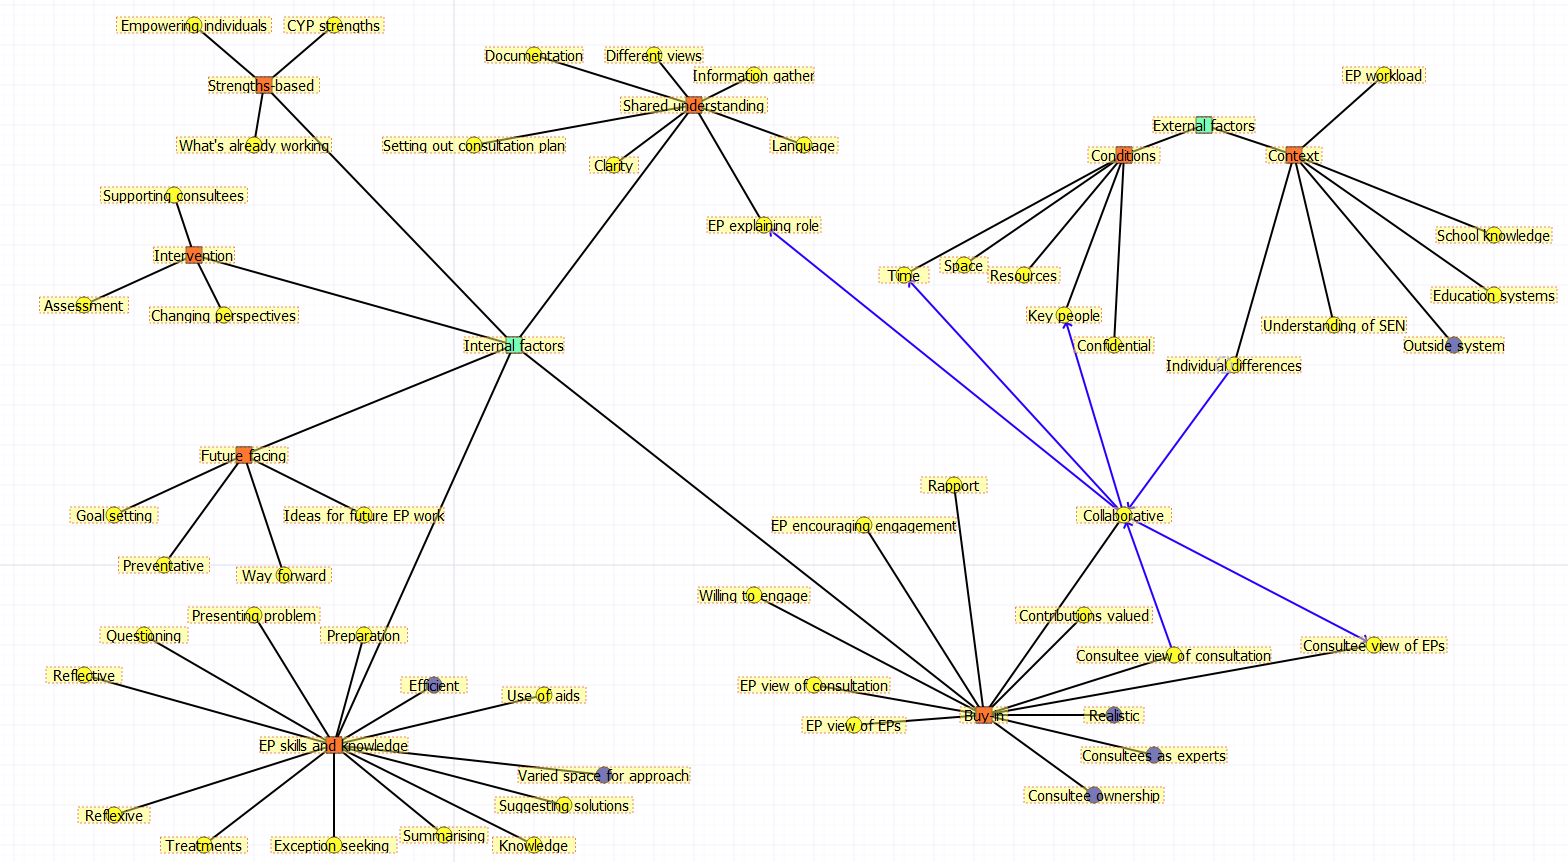
\includegraphics{D:/Doctorate/Assessments/Y3/Thesis/Results/Interview_transcripts/Figures/Thematic_map.png}
\caption{Thematic map}
\end{figure}

\elandscape

\hypertarget{interviews-3}{%
\subsection{3.1 Interviews}\label{interviews-3}}

Thematic analysis identified 32 inductive codes, as well as the 15
deductive codes previously set, relating to what features EPs believed
were effective for consultation. 6 codes were identified for what made
said features effective (see Appendix XXX for the definitions of the
inductive codes, Appendix XXX for the definitions of the codes relating
to what makes the features effective and Appendix XXX for the breakdown
of the number of interviews which each code was identified in and the
total number of codes for each feature). These were combined to create 8
themes: Buy-in, Conditions, Context, Strengths-based, Shared
understanding, Intervention, Future facing, and EP skills and knowledge.
These could then be combined to create two super themes: Internal
factors (features relating to the factors endemic to a consultation) and
External factors (features relating to things happening around a
consultation).

\hypertarget{buy-in}{%
\subsubsection{3.1.1 Buy-in}\label{buy-in}}

This theme related to the importance of EPs creating a bond with those
involved, including the consultee(s) and other school staff members not
directly involved in the consultation, and using this relationship to
facilitate change.

\hypertarget{collaborative}{%
\paragraph{3.1.1.1 Collaborative}\label{collaborative}}

One of the fundamental and most oft cited features for creating buy-in
was making consultation collaborative. Within the consultation, this was
achieved through a variety of factors. One of the key ones was making
sure there was equal participation, such that everyone had a voice and
different perspectives were heard: \emph{``effective consultation
shouldn't being a meeting where one person dominates, whether that may
be a psychologist or anyone else''} (Interview 11) and \emph{``it's like
we're all involved, we're all at the same level, we just come at it from
a different perspective''} (Interview 7).

As a result of there being equal participation, there is a greater
chance that everyone involved has the same understanding of the
situation and the CYP: \emph{``to bring everyone together, and to
co-create and co-construct a shared narrative''} (Interview 11).
Misunderstandings can be cleared up (Interview 5) and these help
everyone feel involved in the process and ensure that the consultation
is collaborative. The creation of a shared narrative can also include
the the creation of a shared agenda. This helps guide the consultation
so it is more effective as it is meeting the needs of those involved and
everyone agrees to it: \emph{``I think a really fundamentally important
part of that consultation is ensuring that we do have that shared
agenda; we know why we're there together and we all agree what we're
doing there together''} (Interview 24) and \emph{``to arrive at a joint
action plan, joint for the school and the parents, school are always
involved as well, so it's more collaborative''} (Interview 10).

This shared agenda can be established by identifying what everyone is
hoping to get from the consultation:

\begin{quote}
\emph{\ldots it would always start with a question about what are your
best hopes from our meeting together? What are your best hopes from our
work together? Because if we don't start with that question, erm, then
we don't know where we're trying to get to. (Interview 27)}
\end{quote}

By working collaboratively with those involved, EPs can facilitate
collaboration between the home and school. This can potentially support
both by helping maintain morale and creating a sense of shared
responsibility:

\begin{quote}
\emph{\ldots there is something that goes on often, not always, in the
room when you've got the family, and school together, the, you do you do
bring that sense of, `We are working on this together; you are not alone
school in this, you are not alone parents in this, we are doing this
together.' (Interview 5)}
\end{quote}

\hypertarget{contributions-valued}{%
\paragraph{3.1.1.2 Contributions valued}\label{contributions-valued}}

A related code, and one which can facilitate a collaborative
consultation, is the idea that everyone who is present in the
consultation should feel able to contribute. Not only this, but they
need to believe that what they say will be taken on board:

\begin{quote}
\emph{\ldots where I would like to think that their views, their
knowledge, their understanding is just as valid as mine\ldots{} we are
equal participants in this. (Interview 13)}
\end{quote}

\begin{quote}
\emph{\ldots equal participation, you know, as far as possible, or that
everybody participates and that everybody feels valued, everybody feels
that what they had to say is useful. (Interview 20)}
\end{quote}

This can help give power to those who may not typically have it in the
school environment, thus helping create a more level playing field and
therefore a more collaborative consultation: \emph{``schools are by
nature very hierarchical. So if you've got a TA they're often not seen
as the same as\ldots{} a SENCO or a head teacher's views but in that
situation they are.''} (Interview 1)

\hypertarget{encouraging-engagement}{%
\paragraph{3.1.1.3 Encouraging
engagement}\label{encouraging-engagement}}

Removing power dynamics within a consultation was seen by many
participants as an important part of the EPs role within consultation.
This formed part of the code `EP encouraging engagement.' The EP must
try and create a space so no consultee feels intimidated and in which
all relevant people can contribute, even if they cannot physically be
present:

\begin{quote}
\emph{\ldots the psychologist trying to level power dynamics is a really
key, a really key part of any consultation and that erm that's in
relation to ourselves, as a professional with a doctorate normally, but
also in relation to the family and the teacher, or the family and the
school. (Interview 2)}
\end{quote}

\begin{quote}
\emph{\ldots balance of people's voices in the rooms. So, erm, making
time for those that might not be able to be present in the meeting to
hear their views and voices. (Interview 27)}
\end{quote}

This code related to any effort by the EP to attempt to include the
voices of the relevant parties. One of the ways that this is through
\emph{``active listening''} (Interview 1). A key idea related to the EP
facilitating others to participate:

\begin{quote}
\emph{I'm there to help facilitate the group in thinking about ways
forward. (Interview 15)}
\end{quote}

\begin{quote}
\emph{\ldots giving a space where people can listen to other people's
perspectives, then you take away the bulk of what it is that you're,
erm, using to try and make a difference. (Interview 21)}
\end{quote}

Not only does the EP need to facilitate others, but also challenge
potentially harmful narratives and navigate difficult situations:

\begin{quote}
\emph{Being careful and being prepared to challenge. (Interview 25)}
\end{quote}

\begin{quote}
\emph{\ldots sometimes a kind of mediation role because\ldots{} we work
in complex and messy situations. And it's not always that people are
going to agree, or even really want to hear what they have to say. So
there's that kind of control in the, the floor that happens in a
consultation, which doesn't happen in other types of conversation.
(Interview 3)}
\end{quote}

Being able to read body language was identified by a few EPs as being
important for facilitating engagement:

\begin{quote}
\emph{you try to do an online meeting, you lose the gesticulations, you
lose\ldots{} being able to point at things or being able to\ldots{} look
at their faces better and realise, `Oh, they're not understanding, I
need to change the way I'm explaining it' or something. I think you lose
so much because it's that non-verbal feedback that you get, that allows
you to know where you are at with the relationship, to know the way you
can develop within that consultation. (Interview 24)}
\end{quote}

However, this was not universal. A few EPs found that using
technologically-mediated (tech) consultations did not lead to a decrease
in quality of the relationship. One EP experienced her consultees asking
for telephone consultations and that these were effective (Interview
16).

\hypertarget{rapport}{%
\paragraph{3.1.1.4 Rapport}\label{rapport}}

The difference between in-person and tech consultations relates to
another core feature, which is the development of a rapport with those
involved in consultations. Within the consultation, an EP must quickly
develop a rapport so that the consultees feel comfortable talking about
potentially difficult topics:

\begin{quote}
\emph{\ldots trust and credibility and shared mutual respect, I think
are at the core of any consultation. You know, they value what I offer
because I'm in touch and the fact they get on well with me, that almost
therapeutic relationship. (Interview 7)}
\end{quote}

\begin{quote}
\emph{\ldots built up that trust and sense of safety, that it's okay to
express their worries, that you can get quite a lot of information.
(Interview 10)}
\end{quote}

The EP needs to not only develop a rapport with those involved, but
encourage relationships between consultees: \emph{``building attuned
interactions in a meeting with parents, with teachers, and then
hopefully between them as well. It just kind of gets everyone on the
same page, hopefully gets everyone pointing in the right direction''}
(Interview 30). This is especially important when relationships between
the home and school have broken down: \emph{"sometimes you have a
breakdown between parents and the school\ldots{} you can be a person in
between, and try and get that working through that\ldots{} which
is\ldots{} a key feature of consultation. (Interview 4)}

Several EPs talked about the importance of having a good relationship
with the school. A good relationship between the school (generally
understood to mean at least the SECNCos and potentially Senior
Leadership Team) helps consultation to be more effective: \emph{"If it's
going to be successful model in a school, I think the need is\ldots{}
time for the EP to build a relationship with the school is important.}
(Interview 23). The reason the relationship is crucial for improving
consultation is that when the EP has developed a good relationship with
the school and they are mutually supporting one another, it is easier to
create an environment which fosters collaboration:

\begin{quote}
\emph{\ldots when you know the school especially, and they're supporting
you in supporting the parents and the staff to do that, then you see it
a lot more". (Interview 1)}
\end{quote}

\begin{quote}
\emph{\ldots schools are often hesitant to adopt consultation as the
main method of EP work: some of the SEN schools that I work with have a
very rigid way of seeing the EP role and what we do, and they're,
they're view is, more often than not, my role as an EP is to go in, do
an assessment, write a report, and that's it. Er, so in those instances,
I find it much harder to sell consultation as a, as a model. (Interview
11)}
\end{quote}

However, several EPs spoke of using their relationship with the school
to change how they approach EP work and what the EP can do in the
school:

\begin{quote}
\emph{\ldots once you build a relationship with schools, and you've been
working in it, you can shift things, you can move things around, to, you
know, working with a bit more control, getting them to see how, you
know, it can be more effective, working with consultation, not doing
just lots of assessments. (Interview 4)}
\end{quote}

\begin{quote}
\emph{That's how you change it. I think that the relationship is super
important. (Interview 23)}
\end{quote}

\hypertarget{ep-view-of-consultation-and-consultee-view-of-consultation}{%
\paragraph{3.1.1.5 EP view of consultation and Consultee view of
consultation}\label{ep-view-of-consultation-and-consultee-view-of-consultation}}

An important feature of consultation that relates to rapport is the
understanding that the consultees, EP, and school as a whole have
towards consultation. How the EP and consultees view consultation can
have a large impact on a consultation and its efficacy. A belief shared
by many interviewees was that \emph{``both parties, kind of, know how
consultation works''} (Interview 24) and this \emph{``might depend on
people's constructs of what consultation is''} (Interview 29).
Interviewees had an overwhelmingly positive view of consultation,
highlighting its versatility and alignment with their values:

\begin{quote}
\emph{\ldots consultation, I think, is a, is a framework with the
complexity that matches the complexity of the concerns that are being
raised. Erm, we're looking at concerns at an individual and a group and
a systemic level. (Interview 21)}
\end{quote}

\begin{quote}
\emph{I don't think you can be inclusive without using a consultative
model. (Interview 25)}
\end{quote}

Though many interviewees identified the value of consultation and the
importance of clearly understanding it and what it involves, many also
pointed out that there is a large heterogeneity of practice among EPs:
\emph{``I think that concept of what a consultation is will vary from
one EP to another''} (Interview 24). There are also EPs who do not value
it and prefer a more traditional style of assessing CYP and then writing
a report. As one interviewee said: \emph{``I know there's a lot of EPs
out there that continue to work in that way and I think, I think that's
one of the barriers to shifting more to a consultation framework''}
(Interview 17). One interviewee, who had recently attended a course on
consultation provided by their EPS, stated:

\begin{quote}
\emph{I'm not sure a lot of EPs really understand what it is. Being able
to communicate that\ldots{} even on that consultation course that I
mentioned I went on, I was really surprised that people, people very
open and very honest, and they said, `We've been saying we've been using
consultation, but we actually have not. We've realised now that we
haven't really been using consultation.' (Interview 22)}
\end{quote}

This makes it difficult for consultees to gain a clear understanding of
what consultation is and has led a few EPs to call for clearer
communication and \emph{``being better at communicating\ldots{} what it
is and what it can do''} (Interview 22). One of the reasons it is
important consultees understand what consultation means is so they can
see the value in it. Many interviewees described how some of the schools
they work in do not appreciate it fully:

\begin{quote}
\emph{\ldots if I could click my fingers and change something on a
systemic level, it would be the attitude toward consultation because I I
really view them as an investment. If you invest in a consultation,
you're going to get better work and and outcomes. Whereas, sometimes
they can be viewed as an expensive hurdle you have to get over to get a
standardised score. (Interview 2)}
\end{quote}

\begin{quote}
\emph{I think there are some schools that, erm, have a negative view of
consultation. Because of that. It's, it's more complex procedure I
think, people realise. (Interview 10)}
\end{quote}

\begin{quote}
\emph{I think we need to educate our schools more about `This is what
the process is,' because we say in sales blurb `We do a consultation'
and, erm, and then the schools are still stuck in that, kind of, old way
of thinking. (Interview 28)}
\end{quote}

A recurring comment centred around the differences between primary and
secondary schools, with primaries typically being more willing to engage
with them:

\begin{quote}
\emph{\ldots most primary SENCOs are very open to whatever I suggest.
And they're quite open to different ways of working, as long as they
have a report to use as evidence, er, for EP involvement, so it has that
element of of a tick box. But most primary schools are very open to
different ways of looking, I would say, but secondaries definitely
aren't. (Interview 18)}
\end{quote}

\hypertarget{ep-view-of-eps-and-consultee-view-of-eps}{%
\paragraph{3.1.1.6 EP view of EPs and Consultee view of
EPs}\label{ep-view-of-eps-and-consultee-view-of-eps}}

Another relevant strand to the different perceptions of consultations is
how the consultees view EPs and their role. Several interviewees talked
about how they were viewed as gatekeepers to resources or as someone who
would fix the situation independently of any work by the consultees:

\begin{quote}
\emph{\ldots the associations that staff or parents can have of us as
being, kind of, the deciders of resources. So we will go in and we will
say, and we will think we are there to support to think about what we
can do for this child, and they will think we are coming in to say `Yes
you can have any EHCP' or `Yes you can have extra money.' (Interview 1)}
\end{quote}

\begin{quote}
\emph{\ldots if school are new to that way of working and they are used
to having an EP come in and, sort of, tell them what to do. I do notice
that sometimes there's a bit of confusion, er, especially from some
teachers who are, `Why are you asking me, aren't you supposed to tell me
what I need to do?' (Interview 11)}
\end{quote}

The consultee view of EPs also affected how receptive a school is to
consultation because \emph{``it very much comes down to the school's
view of my role''} (Interview 14). Several EPs talked about wanting to
change the views of the consultees in the consultation. ***

How the consultees view the EP can be changed in the consultation
itself: \emph{``You're modelling how psychologists think\ldots{} they
might think a psychologist is on a pedestal or whatever, but you're
modelling that psychologists are like everybody else''} (Interview 7).
To help level this power dynamic, EPs often try to present themselves as
not having a privileged position, as some interviewees talked about
\emph{``not putting themselves in an expert position''} (Interview 27).
This is because \emph{``It's the process of discussion itself, erm, that
leads to, kind of, outcomes, rather than taking on an expert model.''}
(Interview 14). However, a few EPs pushed back against the framing of
the EPs non-expert stance as it can be counter-productive: \emph{``I
think, erm, sometimes EPs can go too far the other way in not being the
expert\ldots{} it's a little bit disingenuous, because sometimes we've
got a lot of good ideas to offer''} (Interview 27). How strongly they
take on the role of the expert was independent of the importance of most
EPs placed on being empathetic and supportive:

\begin{quote}
\emph{\ldots you're in the situation as a human being, but also trying
to be a psychologist as well, and they're quite difficult to do at the
same time. (Interview 14)}
\end{quote}

\begin{quote}
\emph{I think you need to be an ally, and a guide, but not be, `I know
what you should do and you should do this.' (Interview 23)}
\end{quote}

\hypertarget{willing-to-engage}{%
\paragraph{3.1.1.7 Willing to engage}\label{willing-to-engage}}

A feature that almost two thirds of the interviewees identified was the
willingness of the consultees to engage in the consultation process:

\begin{quote}
\emph{\ldots the effectiveness is because of engagement, critical
thinking process thinking, and then plan your own action plans, which
you're also engaged in. (Interview 5)}
\end{quote}

\begin{quote}
\emph{\ldots at the same time, to know that the reason that everyone is
around the table for this consultation is to try and shift that thinking
in some way. And usually, you know, just by nature of showing up
everybody does want that, even if they don't necessarily believe it to
be possible, which is why I think those features of consultation are
effective. (Interview 3)}
\end{quote}

\begin{quote}
\emph{\ldots just general engagement from either the parents or school,
and the willingness to, to change; the willingness to change their
practice. (Interview 5)}
\end{quote}

\hypertarget{consultee-ownership}{%
\paragraph{3.1.1.8 Consultee ownership}\label{consultee-ownership}}

Several interviewees talked about how these features are effective
because they help create a sense of consultee ownership of the
situation. By being collaborativeThe consultees are more likely to buy
into the process of consultation and are therefore more likely to feel
they can be an active agent in supporting the CYP:

\begin{quote}
\emph{\ldots when people are active participants in a process, any
process, they would be more likely to follow through with what has been
agreed in terms of, whether that would be actions, whether that would be
a specific approach that needs to be put in place. (Interview 11)}
\end{quote}

\begin{quote}
\emph{\ldots they retain some sense of ownership and some, er, sense of
responsibility for putting in place what comes next. (Interview 20)}
\end{quote}

\begin{quote}
\emph{\ldots the point of that conversation is to leave something behind
for the people who actually have power to do things and if you don't
have their buy-in, then it's totally pointless. I'm struggling to think
of a method, outside of consultation, where you could get that buy in
and that information share and get to any kind of meaningful endpoint.
(Interview 3)}
\end{quote}

\hypertarget{realistic}{%
\paragraph{3.1.1.9 Realistic}\label{realistic}}

Another commonly discussed mechanism for effective consultations was the
increased chance of realistic recommendations and outcomes being
established. If the ideas generated are more co-constructed and built on
shared knowledge, they are more likely to be feasible:

\begin{quote}
\emph{\ldots it also allows for reality, so if you've, you know,
hopefully you're not getting ideas or strategies that are completely
unworkable. So it should be based within the practice of the class
teacher. So it isn't, you know, somebody coming in and going, `Well, you
need to do this three times a day with, you know, dah, dah, dah, dah,
dah.' (Interview 21)}
\end{quote}

\begin{quote}
\emph{\ldots the feedback we get from parents that things are very
grounded in reality, that the ideas that we're talking about makes sense
because they come from a position of understanding and making sense of
whatever is being brought into the room and, sort of, helping to manage
some of the complexity. (Interview 27)}
\end{quote}

\hypertarget{consultees-as-experts}{%
\paragraph{3.1.1.10 Consultees as experts}\label{consultees-as-experts}}

The final code from this theme relates to treating the consultees as
experts of their own area:

\begin{quote}
\emph{I try to make it collaborative because erm, my stance is that we
all bring our own expertise; they're experts as parents, they're experts
on their child. Erm and as teachers, they're experts on, you know,
teaching that child and teaching in general. (Interview 8)}
\end{quote}

\begin{quote}
\emph{I think they're effective because, we're capitalising on that idea
that people are experts in their own lives. (Interview 22)}
\end{quote}

\hypertarget{ep-skills-and-knowledge}{%
\subsubsection{3.1.2 EP skills and
knowledge}\label{ep-skills-and-knowledge}}

The other most common theme related to the psychological knowledge and
skills EPs need to use when engaging in consultation.

\hypertarget{knowledge}{%
\paragraph{3.1.2.1 Knowledge}\label{knowledge}}

The most common code across all themes was in relation to the models of
consultation and general psychological knowledge that the interviewees
believed EPs needed to have to facilitate an effective consultation. The
\emph{``use of theory and reference to the evidence base''} (Interview
2) was identified as an important effective feature of consultation.
Commonly discussed models and frameworks included being solution-focused
(Interview 1), person-centred (Interview 16), trauma and attachment
informed (Interview 13), and using Wagner's model of consultation
(Interview 17) and the COMOIRA model (Interview 25). Other specific
psychological areas included using principles from Narrative Therapy
(Interview 17), an ecosystemic model (Interview 2), social
constructivism (Interview 6), as well as psychologies such as positive
psychology (Interview 9). Some interviewees saw their role as
\emph{``sharing\ldots{} and disseminating psychological theory''}
(Interview 18) and that consultation ``helped {[}them{]} really use
psychology with {[}their{]} schools'' (Interview 11).

The use of a model was often spoken positively as \emph{``{[}giving{]}
the consultation a structure''} (Interview 11) and for one interviewee
they were the most important part:

\begin{quote}
\emph{\ldots for me, the models of psychology are the number one
priority, they have to be systemic and interactionist so that all
behaviour is seen as a function of the person and the situation. So that
if a concern is being described, we want to be looking at finding out
about what was happening at the time or when it was happening.
(Interview 27)}
\end{quote}

\hypertarget{presenting-problem}{%
\paragraph{3.1.2.2 Presenting problem}\label{presenting-problem}}

Many EPs mentioned specific features within different models. One such
feature was exploring the presenting problem from the problem-analysis
framework
(\protect\hyperlink{ref-monsenAccountableModelPractice1998}{Monsen et
al. 1998}):

\begin{quote}
\emph{\ldots getting an idea of what their main concerns are because
when it feels very big, it's really the problem feels very big, the
issue with the child is very messy. There's a lot going on, it can be
hard to know where to start. So focusing them down is something that I
do where I'm like `What's your main concern?' (Interview 8)}
\end{quote}

This code also involved \emph{``further clarification around the
difficulties''} (Interview 11) and a discussion of ``What are the
conditions around it'' (Interview 12).

\hypertarget{treatments}{%
\paragraph{3.1.2.3 Treatments}\label{treatments}}

Another code relating to the problem-analysis framework was the
discussion of treatments for the CYP. This involved \emph{``planning
recommendations''} (Interview 2) and using the consultation \emph{``as a
space where we can really drill down into exactly what you mean when you
say `A social skills group'\,''} (Interview 2) as you can decide what
the intervention is specifically for.

\hypertarget{suggesting-solutions}{%
\paragraph{3.1.2.4 Suggesting solutions}\label{suggesting-solutions}}

Another frequently mentioned model was the Solution-focused model
(\protect\hyperlink{ref-murphySolutionfocusedCounselingSchools1997}{Murphy
1997}). A key part of this model is suggesting solutions and several
interviewees brought this idea up. These are typically recommendations
\emph{``to be done at home and at school''} (Interview 12) Several EPs
stated they were happy to make recommendations but simultaneously did
not want to dominate the consultation (Interview 11). The importance of
taking on board what the consultees said was also voiced by a few
interviewee so that the EP does not make recommendations that have
already been tried (Interview 13).

\hypertarget{exception-seeking}{%
\paragraph{3.1.2.5 Exception seeking}\label{exception-seeking}}

Another code relating to the Solution-focused model was the discussion
of times when the main difficulty is reduced or absent:

\begin{quote}
\emph{\ldots building all those principles of, yes, psychology that
we're trained with, and we're taught to use: exception seeking
(Interview 24)}
\end{quote}

\begin{quote}
\emph{\ldots finding out about other contexts when it was similar and
other contexts when it was different, so that you're able to hypothesise
about what's happening (Interview 27)}
\end{quote}

\hypertarget{reflective}{%
\paragraph{3.1.2.6 Reflective}\label{reflective}}

A feature mentioned by almost all participants centred around the
importance of being reflective. This included the use of
\emph{``reflective listening''} (Interview 1) and \emph{``{[}checking{]}
back in with people\ldots{} working with them just to understand, have
they progressed on that journey''} (Interview 16). Many interviewees
brought up the importance of checking with the consultees
\emph{``whether we did what we wanted to do, and if not, what still
needs to be done?''} (Interview 21).

The importance of being reflective was not limited to within the
consultation; the structure of consultation itself should also
incorporate reflection:

\begin{quote}
\emph{\ldots it might be nice within models that we have with schools,
if there's a definite agreement that there is follow up or a review, if
it's not by me, if it's by someone in the school, because that, that,
kind of, ensures that what's discussed in the consultation is actually,
you know, implemented and monitored. (Interview 14)}
\end{quote}

\begin{quote}
\emph{I also like to have a consultation as a feedback meeting at the
end to\ldots{} revisit what we've discussed in the first session, and
obviously, by that time, I'll have gathered information from other
sources to use that other information to further inform what is going to
be done about the situation and to answer their referral question.
(Interview 9)}
\end{quote}

This reflective structure extends to the gaining of feedback from
consultees. The importance of feedback was mentioned by several
interviewees, for example: \emph{``we have to treat it as a cyclical
process which has to be reviewed and evaluated so that we can use that
feedback to improve practices''} (Interview 1). Learning from peers
through observation and critical reflection with colleagues was also
highlighted:

\begin{quote}
\emph{I would hope that I'm a reflective practitioner and also, erm,
having other people observe consultation, is really helpful in terms of
trying to figure out, sometimes, what's going on, what made a
difference. (Interview 21)}
\end{quote}

\begin{quote}
\emph{\ldots peer supervision is really helpful in terms of, er, helping
your practice because obviously, you've got all that shared, sort of,
ideas and knowledge and bouncing off each other in the team. (Interview
9)}
\end{quote}

\hypertarget{questioning}{%
\paragraph{3.1.2.7 Questioning}\label{questioning}}

The use of question was discussed by more than half the interviewees,
using questions like \emph{``\,`I wonder what would happen if?' `What do
you think might happen if?'\,''} (Interview 25) to explore possibilities
and develop understanding. More banausic questions are asked to explore
a situation to gain a fuller understanding (Interview 5) as well as
exploring the context (Interview 27). However, as the consultation
progresses, questions can be used to get the consultees to think about
what change would look like for the CYP and how they could go about
achieving it (Interview 8). Not only is the content of the questioning
important, but the manner in which they are asked is a key factor
\emph{``how EPs are asking those questions, and the types of questions
they're asking and, erm, the timing of those questions''} (Interview
15).

\hypertarget{use-of-aids}{%
\paragraph{3.1.2.8 Use of aids}\label{use-of-aids}}

A third of interviewees discussed types of supports that they use in
their consultations. Tools based on person-centred psychology, such as
Planning Alternative Tomorrows with Hope (PATHs) and Making Action Plans
(MAPs), was brought up by Interviewees 16 and 17. The use of metaphors
was endorsed as means to safely explore difficult topics (Interview 12),
as well as \emph{``the Japanese problem-solving fish'' and ``blob
trees''} (Interview 10).

\hypertarget{preparation}{%
\paragraph{3.1.2.9 Preparation}\label{preparation}}

A number of interviewees highlighted the importance of being prepared
for a consultation, where the \emph{``psychologist pools all that
information, formulates the hypothesis, types down what questions they
want to ask''} (Interview 20). This increases the chance of the
consultation being effective:

\begin{quote}
\emph{I think doing really thoughtful preparation is essential to to
effective consultation, and I think sometimes there just isn't time for
that but but really spending some time to think about, you know, what,
what do we know? What what do I, what am I hoping to get out of this?"
(Interview 13)}
\end{quote}

This preparation, of \emph{``being in the right headspace yourself''}
(Interview 13) extends to the consultees as them not being prepared can
hamper the efficacy of a consultation:

\begin{quote}
\emph{I think for a lot of the time, what limits my consultations is,
they're just, sort of, caug- maybe a teacher is, sort of, caught on the
cuff, they weren't really expecting me to meet them there, erm, but
there they are. So they haven't really had time to, sort of, gather
their thoughts beforehand. (Interview 20)}
\end{quote}

\hypertarget{reflexive}{%
\paragraph{3.1.2.10 Reflexive}\label{reflexive}}

Another important feature of an effective consultation was the EP being
reflexive. This involves critically analysing, in the moment,
\emph{``\,`How's my body language affecting the person that I'm speaking
with?' `How did that question go down?' `Was it understood?' Am I
helping this person?'''} (Interview 10). This process involves being
\emph{``flexible and responsive''} (Interview 21) and
\emph{``adaptable''} (Interview 30) which can be inhibited by the use of
a consultation script (Interview 30). One interviewee discussed the
importance of:

\begin{quote}
\emph{\ldots being aware of what's going on in the discussion and what
the function of the discussion might be for the consultee at any one
time. For example, if the adult is clearly struggling with the child,
they might be looking for empathy\ldots{} and understanding, so very
much giving that but recognising that that in itself won't necessarily
move things on. So trying to be aware\ldots{} of what the function of
their use of language is at the time and what they're trying to elicit
from me. (Interview 14)}
\end{quote}

Another interviewee discussed the importance of being sensitive to
\emph{``anything that might be\ldots{} difficult for potentially parents
to talk about''} (Interview 15). This process of being reflexive also
helps prevent the EP \emph{``{[}imposing{]} my construct on the
situation''} (Interview 25).

\hypertarget{summarising}{%
\paragraph{3.1.2.11 Summarising}\label{summarising}}

Several EPs mentioned that summarising or paraphrasing (Interview 19)
what has been said in a consultation is an important feature of
consultation. This includes \emph{``re-speaking back to people what
they've told you''} (Interview 17) and \emph{``{[}giving{]} a summary of
what I think I've heard from the different people''} (Interview 5).

\hypertarget{efficient}{%
\paragraph{3.1.2.12 Efficient}\label{efficient}}

The most frequently cited reason for consultation being effective was
that it is an efficient way of practising. This includes the simple fact
that \emph{``more children get to have EP input''} (Interview 11)
because it is possible to \emph{``talk about multiple students and put
multiple things in place as a result of that {[}consultation{]}''}
(Interview 15). It is a tool to \emph{``gather information from
different sources quickly''} (Interview 2) which helps \emph{``generate,
hopefully accurate as possible, hypotheses''} (Interview 30).
Consultation also can \emph{``effect change at a higher level and a
greater level''} (Interview 12) and there can be a \emph{``ripple
effect\ldots{} across policy level or across class or a group or even a
whole school''} (Interview 16). This means that "sometimes you might
only need one or \emph{two consultation sessions to make some good
change"} (Interview 17).

\hypertarget{varied-space-for-approach}{%
\paragraph{3.1.2.13 Varied space for
approach}\label{varied-space-for-approach}}

Another key mechanism through which consultation is effective is its
versatility. \emph{``Consultation is flexible''} (Interview 21) and a
\emph{``process that evolves all the time''} (Interview 24). They allow
for the use of \emph{``different strategies, different components''}
(Interview 10) to meet the needs of the consultees. Because consultation
can be flexible, it can adapt to a situation and therefore have a
greater chance of a positive impact:

\begin{quote}
\emph{I think the logistics of a consultation can remain the same, but
the impact of a consultation can really vary. And\ldots{} I don't know
how many other tools we have available that that's the case for. So, if
I think about the logistics for doing the BAS, or the logistics for
doing a CBT session, I think that you very quickly become constrained by
the way they were set up, whereas, the logistics for a consultation,
getting some people in a room for a certain amount of time, allows for a
flexibility. So\ldots{} sometimes halfway through a consultation, you'll
discover a piece of information that is crucial and up until now
completely unknown, and you can change tack. (Interview 2)}
\end{quote}

\hypertarget{shared-understanding}{%
\subsubsection{3.1.3 Shared understanding}\label{shared-understanding}}

This theme centres around the importance and ways in which EPs create a
common understanding of the situation between themselves and consultees.
\#\#\#\# 3.1.3.1 Different views

Almost every interviewee brought up the importance of gaining the views
of different people and \emph{``gaining multiple perspectives''}
(Interview 21). This includes \emph{``the voice of the child, voice of
the family, voice of the teacher''} (Interview 17). It is particularly
important to bring the voice of the CYP: \emph{``being quite child
centred\ldots{} bringing the pupil voice into that discussion\ldots{}
{[}as{]} it's often not appropriate to have the student in the room,
especially if they're younger''} (Interview 15). A few interviewees
talked about the importance of gaining the views and including those
with power in the system:

\begin{quote}
\emph{I think in some ways, as well, in consultation, making sure trying
to involve, at some stage or at some level, people within a school or
organisation who hold power. So that might be a head or a deputy head.
Just because they have a lot of power within that system, to reframe.
(Interview 17)}
\end{quote}

\begin{quote}
\emph{\ldots we are trying to become more active within the local
authority as well. And I think that's very important. Because otherwise
if you work as an EP service in isolation, without connects- strong
connections with the senior leadership team within the local authority,
and with the senior leadership team within the schools, nobody's gonna
listen. (Interview 23)}
\end{quote}

Consultation also allows for the \emph{``understanding {[}of{]}
different worlds views, different cultural\ldots{} constructs''}
(Interview 17) and one interviewee stated \emph{``when people start to
tell stories of things, it gives you some quite good insights into how
they think and where\ldots{} they're stuck in their thinking''}
(Interview 12). By gaining different views from consultees, the EP is
better placed to make informed hypotheses (Interview 20). When there is
a disagreement between home and school, consultation is an effective
vehicle to \emph{``bring that\ldots{} discrepancy into the room and
discuss it and see if we can come up with it with a kind of compromise
or a way forward that\ldots{} meets the needs of both parties, and
particularly for the student as well''} (Interview 15).

\hypertarget{information-gather}{%
\paragraph{3.1.3.2 Information gather}\label{information-gather}}

A related code was the EP gathering information not directly related to
the main concern: \emph{``I find a lot out about the child, their
background, and\ldots{} about the parents or family and what's going
went around them''} (Interview 8). This included \emph{``{[}gathering{]}
information from across the four areas of SEND''} (Interview 2). This
helps \emph{``inform {[}their{]} assessment''} (Interview 9). However, a
number of interviewees made the point that consultation is much more
than simply gathering information: \emph{``the word `consultation' might
sometimes be interchangeably used with, actually, what's really an
information gathering process''} (Interview 24).

\hypertarget{clarity}{%
\paragraph{3.1.3.3 Clarity}\label{clarity}}

Over half the interviewees talked about the importance of gaining
clarity in a variety of ways. This included for \emph{``what the process
might look like''} (Interview 20) as well as \emph{``clarifying what
people are saying, what the parent is saying, what the SENCO is saying,
what the class teacher is saying''} (Interview 4). This done in the
service of \emph{``understanding the situation better and exploring and
understanding it better''} (Interview 5). This allows for the EP to draw
these strands together and \emph{``come to some kind of
conceptualisation towards the end''} (Interview 5).

\hypertarget{setting-out-consultation-plan}{%
\paragraph{3.1.3.4 Setting out consultation
plan}\label{setting-out-consultation-plan}}

The establishing, by the EP, of the general structure for the
consultation was cited by more than half the interviewees as an
important feature of consultation. This was often done by exploring with
all those involved \emph{``what we're hoping to get from the meeting,
from the consultation''} (Interview 24) because this \emph{``gives it a
clear direction\ldots{} {[}a{]} frame, {[}a{]} boundary''} (Interview
14). It also helps \emph{``{[}manages{]} everyone's expectations''}
(Interview 14) and allows those involved to know if they have achieved
what they wanted to achieve within the consultation (Interview 13).

\hypertarget{language}{%
\paragraph{3.1.3.5 Language}\label{language}}

Several interviewees brought up the importance of the language used
within a consultation. This had two main strands: potential language
difficulties due to English as a second language and the use of jargon
by the professional. One of the barriers to effective consultation is
\emph{``lack of English language, from parents. It's not always possible
to have a translator\ldots{} and even if you do\ldots{} there are
barriers\ldots{} it's difficult going through a third person. You have
no idea\ldots{} how accurately they're translating''} (Interview 5). The
other facet related to the technical language that is pervades
psychology and how this is understood by the consultees:

\begin{quote}
\emph{It takes a much higher level of skill to have a meaningful
consultation with somebody who does not have\ldots{} the privilege of
having\ldots{} lots of education, and\ldots{} {[}a{]} big vocabulary and
high level of verbal skill, than it does\ldots{} for us to sit around in
a team surrounded by people who are educated to doctorate level\ldots{}
But when you really need to try and get meaningful information in a
respectful way from from somebody who finds language very hard,
that's\ldots{} a whole\ldots{} nother level of professional skill.
(Interview 3)}
\end{quote}

\hypertarget{documentation}{%
\paragraph{3.1.3.6 Documentation}\label{documentation}}

Documentation refers to the making of notes and summarising the contents
of the consultation. One EP stated it was \emph{``{[}their{]} least
favourite part of the job\ldots{} But unfortunately, it's really
important, because I think you've got an opportunity to write down and,
kind of, what they call a narrative, like rescue the words''} (Interview
17). Another expressed more uniformly negative views towards
documentation: \emph{``what\ldots{} will make consultations: not having
to flippin' write them up afterwards, we'd get twice as many
done\ldots{} I don't understand why I'm writing about, the magic happens
in the room''} (Interview 22). However, others were more positive:
\emph{``I think the written record is helpful of a consultation''}
(Interview 5) as it gives another opportunity to give advice at a later
date (Interview 30).

\hypertarget{ep-explaining-role}{%
\paragraph{3.1.3.7 EP explaining role}\label{ep-explaining-role}}

A small number of interviewees stated that making sure the consultees
understand what their role is within the consultation is important:
\emph{``try and clarify what my role is and what it isn't''} (Interview
14). This included \emph{``{[}explaining{]} {[}their{]} involvement''}
(Interview 14) and, to help this process, one interviewee talked about
\emph{``{[}doing{]} role of the EP insets, which we would offer every
year, that talks about consultation and the model of psychology and
what's going to happen in the meeting''} (Interview 27).

\hypertarget{intervention}{%
\subsubsection{3.1.4 Intervention}\label{intervention}}

Another theme which arose was the value of consultation as an
intervention in and of itself. This was done through three mechanisms:
providing a space for the EP to change consultees perceptions;
emotionally supporting consultees, and consultation being part of the
assessment process.

\hypertarget{changing-perspectives}{%
\paragraph{3.1.4.1 Changing perspectives}\label{changing-perspectives}}

One of the main ways in which interviewees talked about changing
perspectives was around \emph{``extending the thought processes of the
people involved''} (Interview 10). A common idea among the interviewees
was that the consultation \emph{``facilitates that process of developing
new meaning and new knowledge around a young person, or whatever the
issue might be\ldots{} reframing the way that people see it, which I
think is a key element of change within consultation''} (Interview 17).
The EP should also help others \emph{``not {[}think{]} about a problem
within a child, but {[}think{]} about a young person and how they
interact with the environment that they are in''} (Interview 13). This
change can also happen at a policy level, as one interviewee stated that
consultation was the best vehicle to help schools become more inclusive
(Interview 23). Consultation can also be used to help realign people's
priorities and view towards those involved. Because of the highly
pressurised nature of the systems we work in, \emph{``family, and school
can quite often fall out of sync and having a conversation together
reminds everyone, they're on the same team''} (Interview 2).

This perspective change was not limited to the consultees views towards
the CYP or situation; it extended to their views of consultation itself.
One interviewee talked about how for \emph{``{[}their{]} schools, once
they were introduced to {[}consultation{]}, and once they tried it, they
really liked it''} and they could appreciate that \emph{``consultation
is a good model''} (Interview 11)

\hypertarget{supporting-consultees}{%
\paragraph{3.1.4.2 Supporting consultees}\label{supporting-consultees}}

Another point many EPs made was that consultations can often be used to
help emotionally contain and provide support for the consultees:
\emph{\ldots there is also something about consultation with schools
that I find that can be emotionally containing for staff who perhaps are
highly distressed (Interview 13)}. These \emph{``therapeutic benefits''}
(Interview 2) in a \emph{``therapeutic style of meeting''} (Interview
22) often come through high levels of \emph{``acceptance and empathy''}
(Interview 13) because often consultees want to \emph{``communicate with
someone\ldots{} how challenging it is for them''} (Interview 17).
However, this was an area in which a few EPs judged that tech
consultations were less effective as \emph{``not being able to be
physically there, as the sounding board, as their containing
person\ldots{} I couldn't be that\ldots{} in a virtual environment''}
(Interview 17)

\hypertarget{assessment}{%
\paragraph{3.1.4.3 Assessment}\label{assessment}}

A few interviewees saw the consultation as \emph{``part of the
assessment process''} (Interview 3) and as a \emph{``powerful way to
carry out assessment''} (Interview 19). This is because consultation can
\emph{``{[}lay{]} the foundation for an application for an EHCP
assessment''} (Interview 2).

\hypertarget{strengths-based}{%
\subsubsection{3.1.5 Strengths-based}\label{strengths-based}}

Another emergent theme centred around the focus of consultation: it
being strengths-based as it focuses on bringing out the skills of the
consultees, highlighting what work is already having a positive impact
for the cYP, and discussing the positive qualities of the CYP.

\hypertarget{empowering-individuals}{%
\paragraph{3.1.5.1 Empowering
individuals}\label{empowering-individuals}}

One of the key features of an effective consultation is \emph{``helping
people to identify their own resources''} (Interview 10) and
\emph{``activate better existing skills and knowledge and competence''}
(Interview 13)

\hypertarget{whats-already-working}{%
\paragraph{3.1.5.2 What's already working}\label{whats-already-working}}

One aspect which was frequently discussed was the exploration of what
was already working for the CYP. Interviewees talked about
``{[}trying{]} to build more of a strengths-based and positive outlook,
and look at what's working well, to shift things on'' (Interview 22) and
``trying to find what has been tried, what has worked'' (Interview 28).

\hypertarget{cyp-strengths}{%
\paragraph{3.1.5.3 CYP strengths}\label{cyp-strengths}}

The exploration of the strengths and positive qualities of the CYP was
also mentioned by several interviewees, such as: ``it's exploring skills
and competencies alongside the problem'' (Interview 27). A common idea
was the consultations help reinvigorate the consultees and using the
skills they already have:

\begin{quote}
\emph{``\ldots{} building on what they potentially knew, but didn't
really know what to do with it and\ldots{} empowering and recognising
that they were potentially able to sort out themselves.'' (Interview
19)}
\end{quote}

\begin{quote}
\emph{``\ldots{} a decent consultation\ldots{} can help them feel
empowered and perhaps a little bit reinfused about what their role could
be.'' (Interview 13)}
\end{quote}

A related idea was the empowering of those the consultees engage with,
as a \emph{``rising tide lifts all boats, in the sense that the person
to whom I can give the consultation will very often generalise the
advice from one case to another, from one session to another,
from\ldots{} one class to another''} (Interview 7)

\hypertarget{future-facing}{%
\subsubsection{3.1.6 Future facing}\label{future-facing}}

The final theme of the super code Internal factors focused on the idea
of the consultation as helping to give a path forward for the
consultees. This included the creation of goals for the CYP and the
nature of consultation helping to prevent problems for other CYP in the
future.

\hypertarget{way-forward}{%
\paragraph{3.1.6.1 Way forward}\label{way-forward}}

Over a third of the interviewees talked about how the nature of an
effective consultation gives consultees a structure for how to move
forward in supporting the CYP: \emph{``it provides a mechanism to think
about the future and to move forwards''} (Interview 15). Through
consultation, the EP can \emph{``elicit change or move people forward in
a positive way''} (Interview 22) as well as identify the relevant
support for the CYP (Interview 5). This is different from identifying
specific goals for the CYP as consultations aren't \emph{``always about
solution finding because ways forwards aren't always solutions''}
(Interview 3).

\hypertarget{goal-setting}{%
\paragraph{3.1.6.2 Goal setting}\label{goal-setting}}

For almost a third of interviewees, the identification of precise
outcomes for the CYP to work towards is an important feature of
consultation:

\begin{quote}
\emph{``\ldots{} for it to be consultation, I think there needs to be a
clear, focus on finding, even if it's not a solution, but on coming up
with a plan and\ldots{} having a clear goal in mind.'' (Interview 11)}
\end{quote}

\begin{quote}
\emph{``\ldots{} {[}a{]} key component is goal setting, actually, and
thinking about futures, and what the next steps would be.'' (Interview
17)}
\end{quote}

However, one interviewee argued that not identifying clear goals does
not \emph{``necessarily make it an ineffective consultation''}
(Interview 3).

\hypertarget{preventative}{%
\paragraph{3.1.6.3 Preventative}\label{preventative}}

Because of the emphasis on upskilling consultees within consultations,
an EP using consultation can help prevent issues arising with other CYP
within the school:

\begin{quote}
\emph{``when you're working with a teacher or with families or with
different staff, actually the learning might be, the focus might be
around a specific child, but actually that learning and that reframing
can then be taken and be used preventatively with other young people or
in the classroom'' (Interview 17)}
\end{quote}

By using consultations in different ways, such as regular features of
school life, \emph{``they would become more preventative''} (Interview
14).

\hypertarget{ideas-for-future-ep-work}{%
\paragraph{3.1.6.4 Ideas for future EP
work}\label{ideas-for-future-ep-work}}

A few interviewees brought up the importance of using consultations to
talk about and negotiate future EP involvement with the CYP (Interview
24). This might include an observation of the CYP in class (Interview
4).

\hypertarget{conditions}{%
\subsubsection{3.1.7 Conditions}\label{conditions}}

The first theme of the super code External factors related to the
conditions of the consultations, including who was involved, how much
time was set aside for the consultation, and the space in which it was
held.

\hypertarget{key-people}{%
\paragraph{3.1.7.1 Key people}\label{key-people}}

Almost every interviewee cited having \emph{``all the key
stakeholders''} (Interview 11) involved in the consultation as a key
aspect. Consultation was widely regarded as an \emph{``indirect service
method''} (Interview 17) so involved working with a range of people,
including \emph{``the SENCO, the class teacher, and both the mum and dad
of that child''} (Interview 11). Many interviewees state that it was
crucial to have \emph{``the person that has most knowledge about the
child''} (Interview 10) or the \emph{``people who are most concerned''}
(Interview 21). This included the person who \emph{``has the most
influence''} (Interview 14) as they will be the person who will
implement the agreed interventions.

A number of interviewees highlighted the importance of bringing the
voice of the CYP into the consultation, either by actively involving
them in the consultation (Interview 21) or through those that know the
CYP well (Interview 15).

Many interviewees identified difficulties with conducting consultations
in secondary schools:

\begin{quote}
\emph{\ldots if you've got multiple people working with a young person,
and actually the more people you have, the less anybody feels any
responsibility for them\ldots{} you're trying to find that person who is
most concerned and actually they don't exist. (Interview 13)}
\end{quote}

\begin{quote}
\emph{\ldots it's very difficult to get parents, teachers, parents and
teachers around the same table, at the same time. (Interview 18)}
\end{quote}

\hypertarget{time}{%
\paragraph{3.1.7.2 Time}\label{time}}

Over two thirds of the interviewees brought up time as an important part
of a consultation. This mainly took the form of interviewees stating
that the biggest barrier to effective consultations was a lack of time
within the consultation, for example: \emph{``I don't think you can
have, say an, effective 20 minute consultation. It's not a
consultation''} (Interview 26). This is because you need time for those
involved to move beyond the ``black and white way of thinking'' about
labels (Interview 18).

A related issue centred around the amount of time bought in by schools.
Because the majority of interviewees either worked for fully traded
services or as private EPs, the schools they worked with only had a
limited amount of contact time. This led to several interviewees
discussing the difficulty of bringing about change with schools because
of the time limits placed on them (Interview 12).

This was an area where tech consultations provided an advantage, as EPs
can save time by not travelling between different schools (Interviews
13, 17, \& 29).

\hypertarget{resources}{%
\paragraph{3.1.7.3 Resources}\label{resources}}

Resources was often cited important feature to consultations. This had
several dimensions, including the ability of the consultees to enact
change for the CYP due to resource constraints:

\begin{quote}
\emph{The biggest barrier I come across is people saying, `Well, that's
lovely and I think we've come up with some fabulous ideas. However, I
don't think management will let me do that'\ldots{} So top down
squashing\ldots{} it's budgetary, it's time-bound, it's people saying,
`Well, we don't have the physical resources to be able to do that.'
(Interview 16)}
\end{quote}

\begin{quote}
\emph{\ldots{} we might have all the ideas in the world around how
someone might be supported. And it doesn't, I guess, affect the
consultation in itself so much but it affects, it does affect the type
of dialogue we might have around, schools and just the lack in, the
workforce, the lack in staff, they're lacking the resourcing to really
support some of these young people in the way that we would like them to
be. I think that shapes consultations. (Interview 17)}
\end{quote}

Another dimension is the resources school have to allow staff the time
off from lessons to fully engage with a consultation: \emph{``schools
thinking `We don't have the time and the capacity to free up staff to
come and, come and sit and have a consultation'\,''} (Interview 15).

A third dimension related to the resources available to the schools to
buy in EP time:

\begin{quote}
\emph{\ldots{} I've certainly got schools that repeatedly say to me that
they would love more EP time but they can't afford it in a traded
environment and lots of\ldots{} competing things that they have to spend
money on. (Interview 21)}
\end{quote}

\hypertarget{space}{%
\paragraph{3.1.7.4 Space}\label{space}}

A number of interviewees identified the importance of creating a space
for effective consultations to occur. This encompassed both the physical
space of the location and the mental space to be able to deal with
complex experiences:

\begin{quote}
\emph{\ldots{} sometimes people have asked to do consultations in rooms
where there are other people and it's just messy. (Interview 2)}
\end{quote}

\begin{quote}
\emph{I think the room that you meet in is quite important and the way
that it's set up\ldots{} so\ldots{} it doesn't seem like an interview
situation. (Interview 9)}
\end{quote}

This aspect is particularly important for tech consultations as these
almost always occur in the EP's and consultee's home:

\begin{quote}
\emph{\ldots{} it can be difficult for staff to really, and parents, to
really engage with the process, if they've got children running around
and things going on. So\ldots{} doing it where they can't have a
separate space, emotionally as well as physically, can be tricky.
(Interview 14)}
\end{quote}

\begin{quote}
\emph{\ldots{} having to make sure that doors are secure, so children
can't run in at particular points. (Interview 24)}
\end{quote}

\hypertarget{confidential}{%
\paragraph{3.1.7.5 Confidential}\label{confidential}}

Several interviewees brought up the importance of confidentiality for
what was discussed in the consultation: \emph{``we want to have a
confidential place to reflect''} (Interview 22). This helps
\emph{``contribute towards building that kind of environment where
people feel happy to share''} (Interview 15). The importance of
confidentiality was made more important for many interviewees by the
unexpected transition to tech consultations in response to the COVID-19
pandemic, with several identifying issues around security, for example:
``the first step is finding an effective platform that's got enough
safety features for us to be able to\ldots{} carry out a consultation''
(Interview 10).

\hypertarget{context}{%
\subsubsection{3.1.8 Context}\label{context}}

The second code within the External factors super theme was related to
the general context that consultations are conducted within.

\hypertarget{education-systems}{%
\paragraph{3.1.8.1 Education systems}\label{education-systems}}

EPs work within many systems. These can all impact on individual
consultations and on how EPs work through consultation. For example,
\emph{``there are schools who don't particularly value
{[}consultation{]} and just want us to do assessments''} (Interview 5).
As one interviewee stated, \emph{``all the work of the EPs is determined
by the context in which it's set and by the organisational agendas in
which it's set''} (Interview 10). Several interviewees talked about the
bureaucracy of the education system impacting on consultations and EP
work as a whole:

\begin{quote}
\emph{\ldots{[}the{]} role of the EP is less problem solving, it's more
ticking a box, more bureaucratic exercise rather than a solving
facilitation. (Interview 10)}
\end{quote}

\begin{quote}
\emph{\ldots there is a bureaucracy around an education, health care
plan, in terms of certain reports being written, certain hurdles being
gone through and certain assessments taking place. And so\ldots{} we're
not doing any thinking, we're merely following a bureaucratic process.
(Interview 6)}
\end{quote}

Other wider systemic issues related to how society as a whole sees
additional needs:

\begin{quote}
\emph{\ldots the medical model is so predominant\ldots{} And I often
find that those explanations for, learning and development and
behaviours, can dominate conversations\ldots{} ADHD, ASD\ldots{} they
are definitely a barrier to creating more effective, positive change.
(Interview 17)}
\end{quote}

\begin{quote}
\emph{\ldots there's enormous pressure, ever increasing pressure on
schools, to get results. And\ldots{} {[}that's{]} antithetical to
consultation. (Interview 25)}
\end{quote}

A number of EPs identified operating in traded services as a barrier to
consultation:

\begin{quote}
\emph{\ldots I feel like it's the situation in which we work, the whole
traded model, which means that consultation is, an addition\ldots{} we
just have to do it to get the information. It's not\ldots{} valued
as\ldots{} a way of working in and of itself. (Interview 8)}
\end{quote}

\begin{quote}
\emph{\ldots I find within a traded service, you're quite constricted,
in lots of ways about what the school expect in terms of the use of your
time. (Interview 9)}
\end{quote}

\begin{quote}
\emph{\ldots I feel like\ldots{} particularly in the traded service
model, that dynamic is really hard to manage. And\ldots{} it's been a
real difficulty to introduce consultation as a working modelling in many
of my schools. (Interview 11)}
\end{quote}

Another issue that was identified was the views that school staff had
towards change because of the people with more power in the system:
\emph{``SENCOs feeling unable to make change because of the head
teacher''} (Interview 23).

\hypertarget{individual-differences}{%
\paragraph{3.1.8.2 Individual
differences}\label{individual-differences}}

Almost five sixths of the interviewees brought up the characteristics of
those involved in the consultation as an important feature of a
consultation. The personalities, histories, and on the day mood of the
consultees will likely impact on a consultation:

\begin{quote}
\emph{\ldots{} that's going to play out in the room, in different ways,
depending on the circumstances, the resilience of individuals, position,
their own history, etc, etc. And will play out differently day to day,
with the same people. (Interview 25)}
\end{quote}

\begin{quote}
\emph{\ldots{} there are parents who just don't like coming into school,
are barred from school\ldots{} have such a difficult relationship with
school that is not possible. Physically can't get there because of
health issues or younger children. (Interview 5)}
\end{quote}

\begin{quote}
\emph{I think there's always going to be a level of\ldots{} personality
involved, that with some people, it is easier to\ldots{} get
that\ldots{} feeling of engagement higher than it is with others\ldots{}
I think there is some variability, just because of human nature and the
different personalities of the people that you meet. (Interview 12)}
\end{quote}

The personality of the EP was identified by a few interviewees as
potentially impacting on a consultation, for example: \emph{``I think
the personality of the individual EP can have a big impact''} (Interview
24). EP confidence in their own skill and knowledge was also identified
as an important feature (Interview 14).

This variability in the presentation of consultation was viewed as a
potential negative for consultation; if a teacher or parent was told
they had to attend a consultation they \emph{``wouldn't know what to
expect because it would depend so much on the individual''} (Interview
11) because \emph{``everybody has gone on their own and done totally
different things''} (Interview 23).

\hypertarget{understanding-of-sen}{%
\paragraph{3.1.8.3 Understanding of SEN}\label{understanding-of-sen}}

A few interviewees stated that the way a school understands additional
needs within an education context can have an impact on consultations.
Some schools cleave to a more traditional `within-child' understanding
of additional needs, particularly secondary schools (Interview 14). As
such, it is much harder to encourage these schools to adopt consultation
as a way of working (Interview 11).

\hypertarget{ep-workload}{%
\paragraph{3.1.8.4 EP workload}\label{ep-workload}}

Almost a third of interviewees identified the amount of work EPs
typically do as being a barrier to effective consultations. This was
because the volume of work prohibits being able to fully engage with a
case:

\begin{quote}
\emph{\ldots{} when you are on the day job, and you are 24-7 doing EP
stuff, and you have\ldots{} a stupid amount of cases and a stupid amount
of schools and you cannot think\ldots{} you are running on\ldots{} empty
(Interview 23)}
\end{quote}

\begin{quote}
\emph{\ldots{} you're so tired and stressed\ldots{} you're not really
thinking as well\ldots{} you can't reflect on it and come up with
different ideas and solutions because\ldots{} you just have to get that
written, get it sent off, and get on to the next thing. (Interview 9)}
\end{quote}

One interviewee identified the positive benefit of moving to tech
consultations because \emph{``I have a lot more time in my day, which
means that I actually have a lot more space to think about children and
cases''} (Interview 18).

\hypertarget{school-knowledge}{%
\paragraph{3.1.8.5 School knowledge}\label{school-knowledge}}

A few interviewees stated that having \emph{``in depth knowledge of
schools and how they work''} (Interview 7), in particular secondary
schools (Interview 22), helped their consultations be more effective.
One interviewee explained that having good knowledge of the whole system
differentiated EPs from clinical psychologists because EPs are
``fluent\ldots{} in that\ldots{} understanding and situational context''
(Interview 21).

\hypertarget{outside-system}{%
\paragraph{3.1.8.6 Outside system}\label{outside-system}}

Almost a third of interviewees stated that the EP working outside the
school system helped their consultations be more effective:

\begin{quote}
\emph{I think being an external person helps\ldots{} you are able to ask
some of the questions of parents that school can't, you can also ask
questions of school that parents {[}can't{]} and take on that more
challenging aspects. (Interview 5)}
\end{quote}

\begin{quote}
\emph{\ldots{} we have to get meta to the situation and not get too
bogged down and immersed in the nitty gritty. So keeping meta and
keeping perspective on it, I think is a skill that EPs can bring, that
really helps. And that's the beauty of not working in the system, is the
beauty of going in and out of schools. (Interview 27)}
\end{quote}

POTENTIALLY USE ELSEWHERE The EP is gathering and summarising the ideas
and saying, `Given what we've discussed, and the ideas we've heard so
far, what is going to make most sense for this young person and what's
going to make most difference?' And then it's getting the ideas from the
people. (Interview 27)

Collaboration was identified as a key factor not only because it
increased the consultee's willingness to engage but because it increased
the chances of the recommendations being put in place:

I think if you have a really good consultation and you can actually
problem solve together, and the people that you're consulting with,
actually come up with some of the ideas, then it's much more likely for
those interventions to happen. (Interview 20)

it underpins all of the work that we do with schools. So I would say
every school visit, team meetings, organisational level consultations,
we would be applying the same psychologies, the same frameworks.
(Interview 27)

\hypertarget{section}{%
\paragraph{}\label{section}}

\hypertarget{questionnaire}{%
\subsection{3.2 Questionnaire}\label{questionnaire}}

\hypertarget{observations-1}{%
\subsection{Observations}\label{observations-1}}

No pair-wise simplifications could be made as there were no
consultations which saw change which differed by only 1 feature.

\begin{longtable}[]{@{}llrlrrrr@{}}
\caption{TME goals with ratings for baseline, expected, and
actual}\tabularnewline
\toprule
EP & Adult & Child & Goal & Baseline & Expected & Actual & Change \\
\midrule
\endfirsthead
\toprule
EP & Adult & Child & Goal & Baseline & Expected & Actual & Change \\
\midrule
\endhead
1 & Teacher & 1 & Maths problems up to 10 & 3 & 6 & 4 & 1 \\
1 & Teacher & 1 & Accept play requests & 3 & 5 & 4 & 1 \\
1 & Parent & 1 & Maths problems up to 10 & 3 & 5 & 3 & 0 \\
2 & Teacher & 2 & Not pausing when naming emotions & 3 & 7 & 3 & 0 \\
2 & Parent & 2 & Using phoneme knowledge for unfamiliar words & 5 & 8 &
7 & 2 \\
2 & Parent & 2 & Maintaining a conversation & 3 & 5 & 4 & 1 \\
2 & Parent & 2 & Not pausing when naming emotions & 5 & 8 & 6 & 1 \\
2 & Parent & 3 & Learning self-esteem & 3 & 4 & 3 & 0 \\
2 & Teacher & 4 & Learning self-esteem & 2 & 4 & 3 & 1 \\
2 & Parent & 4 & Managing frustration when instructed & 3 & 5 & 4 & 1 \\
\bottomrule
\end{longtable}

\hypertarget{discussion}{%
\section{Discussion}\label{discussion}}

Buy-in was facilitated by the EP not taking an expert stance and
creating a collaborative and sharing environment for the consultees to
explore their thoughts.

There was a large disparity between the number of inductive and
deductive codes and the number of instances of each code, with the
inductive codes being recorded more frequently than deductive codes.
This suggests that the current literature does not accurately reflect
how EPs are using consultation in practice.

Observations were almost exclusively from one EP.

No measures were taken to ensure the reliability of the thematic
analysis, such as using inter-rater reliability.

\hypertarget{appendices}{%
\section{Appendices}\label{appendices}}

\hypertarget{appendix-1}{%
\subsection{Appendix 1}\label{appendix-1}}

\begin{longtable}[]{@{}llll@{}}
\toprule
Consultation number & Child & EP & Consultees \\
\midrule
\endhead
1 & 1 & 1 & Mother and teacher \\
2 & 2 & 2 & Father \\
3 & 2 & 2 & Teacher \\
4 & 3 & 2 & Mother \\
5 & 4 & 2 & Teacher \\
6 & 4 & 2 & Father and father \\
\bottomrule
\end{longtable}

\hypertarget{appendix-2}{%
\subsection{Appendix 2}\label{appendix-2}}

\begin{enumerate}
\def\labelenumi{\arabic{enumi})}
\tightlist
\item
  What is your role?
\item
  How do you define consultation? What does it mean to you?
\item
  What key words would you use?
\item
  How often have you engaged with consultation?
\item
  What history of consultation training do you have?
\item
  Does your current EPS value consultation/operate a consultation-based
  service?
\item
  Why do you use consultation?
\item
  What do you believe are the key features of a consultation? What needs
  to be present for it to be more than a conversation?
\item
  What features do you most frequently see (what is seen may be
  different what they believe is effective)?
\item
  What do you believe are the key features of an effective consultation
  (including examples)?
\item
  What makes them effective?
\item
  How could consultations be more effective?
\item
  What are the barriers to effective consultation?
\item
  If you could not use consultation, what work would you use instead?
\item
  What is the unique contribution of consultation?
\item
  What has changed with regards to your consultation work during
  lockdown?
\item
  How have you found this change?
\item
  Advantages/disadvantages?
\item
  Will you do anything differently after this is over?
\item
  Should the service/EPs as a whole do things differently?
\end{enumerate}

\hypertarget{appendix-3}{%
\subsection{Appendix 3}\label{appendix-3}}

\begin{longtable}[]{@{}
  >{\raggedright\arraybackslash}p{(\columnwidth - 2\tabcolsep) * \real{0.47}}
  >{\raggedright\arraybackslash}p{(\columnwidth - 2\tabcolsep) * \real{0.51}}@{}}
\toprule
Category & Definition \\
\midrule
\endhead
Info gather & Fact finding or discussion of non-key concern(s). \\
Suggesting solutions & The EP volunteering a solution to the presenting
concern. \\
CYP strengths & Any discussion of the CYP's positive qualities:
attributes, personality, actions, etc. \\
Discussing what's already working & Discussion (including evaluation) of
any intervention/change which has improved the current situation for the
CYP. \\
Everyone's contributions valued & Consultees giving their view on
something e.g.~presenting hypotheses, suggesting solutions, or the EP
explicitly acknowledging someone for their contribution. Not just the
consultee(s) speaking/giving an answer to a factual question. \\
Understanding presenting problem & Discussion of any aspect of the main
presenting concern(s) including scope, environmental factors,
exceptions, etc. and why a problem may be present
(\protect\hyperlink{ref-sheridanSchoolConsultation2000}{S. Sheridan,
Richards, and Smoot 2000}) \\
Summarising & The EP saying back what has previously been stated by
consultees in the consultation (potentially building on it but not
necessarily). \\
Planning/implementing treatments & Discussion and agreement between the
consultant and consultee on any interventions that will be implemented
to support the CYP
(\protect\hyperlink{ref-sheridanSchoolConsultation2000}{S. Sheridan,
Richards, and Smoot 2000}). \\
EP using expert knowledge & EP discussing topics which they have
knowledge of (from both professional experience and academic reading)
within school psychology theory and practice. \\
EP explaining role & EP explicitly talking about the work of an EP and
its purpose. \\
Setting out plan for consultation & Discussion of what will happen over
the course of the consultation. \\
Ideas for future EP work & Discussion of potential work an EP can do in
the future, such as consultation, assessment, observation, etc. \\
Empowering individuals & Any comments or questions which aim to increase
the skills of the consultees (teachers, parents, SENCOs,
etc.)/upskilling consultees so they can solve their problems
(\protect\hyperlink{ref-nolanProcessPsychologicalConsultation2014}{Nolan
and Moreland 2014}). \\
School knowledge & Any comments or questions which increase
understanding of how the school works. \\
\bottomrule
\end{longtable}

\hypertarget{appendix-4}{%
\subsection{Appendix 4}\label{appendix-4}}

\begin{longtable}[]{@{}
  >{\raggedright\arraybackslash}p{(\columnwidth - 2\tabcolsep) * \real{0.35}}
  >{\raggedright\arraybackslash}p{(\columnwidth - 2\tabcolsep) * \real{0.64}}@{}}
\toprule
Level & Feature \\
\midrule
\endhead
Solution-focused & Suggesting solutions; Highlighting the strengths of
the CYP; Discussing what is already working; Exploring exceptions;
Suggesting ideas for future EP work. \\
Problem analysis & Fully understanding the presenting problem; How to
implement the interventions \\
Organisation and knowledge & Gathering information; Summarising; Using
knowledge; Setting out a plan; Explaining what EPs do; School
knowledge \\
Valuing everyone & Everyone contributing; empowering those involved \\
\bottomrule
\end{longtable}

\hypertarget{appendix-5}{%
\subsection{Appendix 5}\label{appendix-5}}

\begin{longtable}[]{@{}
  >{\raggedright\arraybackslash}p{(\columnwidth - 2\tabcolsep) * \real{0.35}}
  >{\raggedright\arraybackslash}p{(\columnwidth - 2\tabcolsep) * \real{0.64}}@{}}
\toprule
Code & Definition \\
\midrule
\endhead
Assessment & How consultation can be a form of assessment. \\
Changing perspectives & Any discussion of the EP changing the
perspectives of consultees during consultation or the understanding of
consultation by consultees. \\
Clarity & Gaining clarity regarding the issues through formulation
etc. \\
Collaborative & Any discussion of a joint or collaborative aspect of
consultation. \\
Confidential & Confidentiality and privacy \\
Consultee view of consultation & How the consultees view consultation
and understand it, as well as discussion of increasing understanding
through training. \\
Consultee views of EPs & How the consultee views the role of the EP,
including as the expert. \\
Different views & Gaining the views of a variety of different people,
including the young person, to explore narratives and triangulate
evidence. \\
Documentation & Writing of notes or reports which detail what
happened. \\
Education systems & How the school systems and bureaucratic processes of
the British education system impact consultation. \\
EP encouraging engagement & The EP being engaged in the consultation
through active listening to challenge narratives and facilitate
discussion. \\
EP view of consultation & The EPs understanding of consultation. \\
EP view of EPs & The EPs understanding of their role, including as the
expert. \\
EP workload & How the high workload EPs experience impacts
consultation. \\
Goal setting & Explicit discussion of outcomes and goal setting. \\
Individual differences & How the personalities and histories of the
consultees and consultors impacts consultation. \\
Key people & Having the people who are most concerned present. \\
Language & Using language that can be understood by all as well as
issues regarding English as an Additional Language. \\
Preparation & Time for the consultees and consultors to prepare. \\
Preventative & How consultation can help prevent issues arising or
exacerbating. \\
Questioning & Use of a wide range of questions within consultation for a
multitude of purposes, including to explore and challenge. \\
Rapport & The importance of relationships with those involved and how it
can be developed. \\
Reflective & Reflecting on an individual consultation, receiving
feedback, or having a review consultation to explore how the situation
has progressed. \\
Reflexive & In consultation checking, by the EP, of how they and others
might be affected by the discussion as well as what they are saying and
why. \\
Resources & How a lack of resources from the school can impact on
consultation, including not giving teachers enough time for them. \\
Space & Having both the physical and mental space to engage with
consultation. \\
Supporting consultees & EPs providing therapeutic support for consultees
during a consultation. \\
Time & Having enough time within the consultation to maximise its
use. \\
Understanding of SEN & How consultees and schools see special
educational needs in children and how it impacts consultation. \\
Use of aids & Using aids such as Planning Alternative Tomorrows with
Hope etc. \\
Way forward & General statements about how consultation can provide a
way forward. \\
Willing to engage & Consultees being willing to engage with the process
of consultation. \\
\bottomrule
\end{longtable}

\hypertarget{appendix-6}{%
\subsection{Appendix 6}\label{appendix-6}}

\begin{longtable}[]{@{}
  >{\raggedright\arraybackslash}p{(\columnwidth - 2\tabcolsep) * \real{0.35}}
  >{\raggedright\arraybackslash}p{(\columnwidth - 2\tabcolsep) * \real{0.64}}@{}}
\toprule
Code & Definition \\
\midrule
\endhead
Consultee ownership & Consultees having a sense of responsibility for
what will happen next to support the CYP. \\
Consultees as experts & Viewing consultees as experts in the lives of
the child or as teachers of the child who have valuable knowledge to
share. \\
Efficient & Being able to impact at multiple levels, over time, and have
wide ranging impacts. \\
Outside system & EPs being outside the school system giving them a meta
perspective, a new way of seeing things, which allows them to challenge
and explore. \\
Realistic & The recommendations made are realistic to the setting and
capabilities of those involved, including regarding resources, and are
time bound. \\
Varied space for approach & Consultation being a highly flexible vehicle
to support CYP. \\
\bottomrule
\end{longtable}

\hypertarget{appendix-7}{%
\subsection{Appendix 7}\label{appendix-7}}

\begin{longtable}[]{@{}lll@{}}
\toprule
Code & File n & Total code n \\
\midrule
\endhead
Everyone's contributions valued & 14 & 33 \\
CYP strengths & 7 & 9 \\
Empowering individuals & 19 & 68 \\
Exception seeking & 5 & 8 \\
EP explaining role & 5 & 5 \\
Ideas for future EP work & 4 & 4 \\
Information gathering & 18 & 48 \\
EP using expert knowledge & 30 & 223 \\
Understanding presenting problem & 16 & 35 \\
School knowledge & 3 & 4 \\
Setting out plan for consultation & 16 & 31 \\
Suggesting solutions & 11 & 14 \\
Summarising & 6 & 7 \\
Planning/ implementing treatments & 8 & 15 \\
Discussing what's already working & 11 & 21 \\
Assessment & 5 & 14 \\
Changing perspectives & 25 & 118 \\
Clarity & 17 & 37 \\
Collaborative & 29 & 212 \\
Confidential & 10 & 13 \\
Consultee view of consultation & 28 & 155 \\
Consultee views of EPs & 26 & 84 \\
Different views & 27 & 150 \\
Documentation & 8 & 10 \\
Education systems & 27 & 134 \\
EP encouraging engagement & 29 & 119 \\
EP view of consultation & 22 & 77 \\
EP view of EPs & 14 & 28 \\
EP workload & 7 & 16 \\
Goal setting & 13 & 21 \\
Individual differences & 24 & 47 \\
Key people & 27 & 81 \\
Language & 8 & 13 \\
Preparation & 10 & 22 \\
Preventative & 5 & 5 \\
Questioning & 19 & 43 \\
Rapport & 26 & 91 \\
Reflective & 26 & 110 \\
Reflexive & 9 & 21 \\
Resources & 15 & 22 \\
Space & 15 & 20 \\
Supporting consultees & 12 & 27 \\
Time & 22 & 61 \\
Understanding of SEN & 3 & 7 \\
Use of aids & 10 & 22 \\
Way forward & 13 & 22 \\
Willing to engage & 19 & 41 \\
Consultee ownership & 15 & 27 \\
Consultees as experts & 5 & 6 \\
Efficient & 18 & 43 \\
Outside system & 8 & 12 \\
Realistic & 7 & 11 \\
Varied space for approach & 10 & 15 \\
\bottomrule
\end{longtable}

\hypertarget{references}{%
\section*{References}\label{references}}
\addcontentsline{toc}{section}{References}

\hypertarget{refs}{}
\begin{CSLReferences}{1}{0}
\leavevmode\hypertarget{ref-aepSurveyEffectsCovid192020}{}%
AEP. 2020. {``Survey into the Effects of {Covid}-19 on the Provision of
Educational Psychology Services in {England}.''}

\leavevmode\hypertarget{ref-andrewsSelfReportToolsCompare2015a}{}%
Andrews, Sally, David A. Ellis, Heather Shaw, and Lukasz Piwek. 2015.
{``Beyond {Self}-{Report}: {Tools} to {Compare Estimated} and
{Real}-{World Smartphone Use}.''} \emph{PLOS ONE} 10 (10): e0139004.
\url{https://doi.org/10.1371/journal.pone.0139004}.

\leavevmode\hypertarget{ref-argyrisTheoryPracticeIncreasing1992}{}%
Argyris, Chris, and Donald A. Schon. 1992. \emph{Theory in {Practice}:
{Increasing Professional Effectiveness}}. 1 edition. {San Francisco}:
{Jossey-Bass}.

\leavevmode\hypertarget{ref-ashtonWhatValuableUnique2006}{}%
Ashton, Rebecca, and Elizabeth Roberts. 2006. {``What Is {Valuable} and
{Unique} about the {Educational Psychologist}?''} \emph{Educational
Psychology in Practice} 22 (2): 111--23.
\url{https://doi.org/10.1080/02667360600668204}.

\leavevmode\hypertarget{ref-bellPerceptionsRealitiesRole2013}{}%
Bell, Henry D., and Vicki McKenzie. 2013. {``Perceptions and
{Realities}: {The Role} of {School Psychologists} in {Melbourne},
{Australia}.''} \emph{The Educational and Developmental Psychologist} 30
(1): 54--73. \url{https://doi.org/10.1017/edp.2013.1}.

\leavevmode\hypertarget{ref-berganBehavioralConsultationTherapy1990}{}%
Bergan, John R., and Thomas R. Kratochwill. 1990. \emph{Behavioral
{Consultation} and {Therapy}: {An Individual Guide}}. 1990 edition. {New
York}: {Springer}.

\leavevmode\hypertarget{ref-bhardwajRapidLiteratureReview2020}{}%
Bhardwaj, Amber, Catherine Byng, and Zoë Morrice. 2020. {``A Rapid
Literature Review of How to Support the Psychological Well-Being of
School Staff During and After {Covid}-19.''}

\leavevmode\hypertarget{ref-boyatzisTransformingQualitativeInformation1998a}{}%
Boyatzis, Richard E. 1998. \emph{Transforming Qualitative Information:
Thematic Analysis and Code Development}. {Thousand Oaks, Calif. ;
London}: {SAGE}.

\leavevmode\hypertarget{ref-braunUsingThematicAnalysis2006}{}%
Braun, Virginia, and Victoria Clarke. 2006. {``Using Thematic Analysis
in Psychology.''} \emph{Qualitative Research in Psychology} 3 (2):
77--101. \url{https://doi.org/10.1191/1478088706qp063oa}.

\leavevmode\hypertarget{ref-britishpsychologicalsocietyQualityStandardsEducational2015}{}%
British Psychological Society. 2015. {``Quality {Standards} for
{Educational Psychology Services} - {Good Practice Guidelines} -
{Publication} by {Series} - {Publications}.''}
https://shop.bps.org.uk/publications/publication-by-series/good-practice-guidelines/quality-standards-for-educational-psychology-services.html.

\leavevmode\hypertarget{ref-bronfenbrennerEcologyHumanDevelopment1981}{}%
Bronfenbrenner, Urie. 1981. \emph{The {Ecology} of {Human Development}:
{Experiments} by {Nature} and {Design}}. Unknown edition. {Cambridge,
Mass}: {Harvard University Press}.

\leavevmode\hypertarget{ref-cabinetofficeStayingHomeAway2020}{}%
Cabinet Office. 2020. {``Staying at Home and Away from Others (Social
Distancing).''} \emph{GOV.UK}.
https://www.gov.uk/government/publications/full-guidance-on-staying-at-home-and-away-from-others/full-guidance-on-staying-at-home-and-away-from-others.

\leavevmode\hypertarget{ref-cicchettiGuidelinesCriteriaRules1994}{}%
Cicchetti, Domenic. 1994. {``Guidelines, {Criteria}, and {Rules} of
{Thumb} for {Evaluating Normed} and {Standardized Assessment Instrument}
in {Psychology}.''} \emph{Psychological Assessment} 6 (December):
284--90. \url{https://doi.org/10.1037/1040-3590.6.4.284}.

\leavevmode\hypertarget{ref-clineQualityAssuranceEducational1994a}{}%
Cline, Tony. 1994. {``Quality {Assurance} in an {Educational Psychology
Service}: {What Can We Learn} from {Earlier Experience} in {Service
Evaluation}?''} \emph{School Psychology International}.
\url{https://doi.org/10.1177/0143034394153002}.

\leavevmode\hypertarget{ref-connorTargetMonitoringEvaluation2010}{}%
Connor, Tom. 2010. {``Target Monitoring and Evaluation : Measuring the
Impact of Educational Psychology Interventions.''} Ph.\{\{D\}\}.,
Institute of Education, University of London.

\leavevmode\hypertarget{ref-cordingStudyEducationalPsychologists2011}{}%
Cording, James. 2011. {``A Study of {Educational Psychologists}' Use of
Consultation and Users' Views on What a Service Should Deliver,''} 158.

\leavevmode\hypertarget{ref-crabtreeTemplateApproachText1992}{}%
Crabtree, Benjamin F., and William F. Miller. 1992. {``A Template
Approach to Text Analysis: {Developing} and Using Codebooks.''} In
\emph{Doing Qualitative Research}, 93--109. Research Methods for Primary
Care, {Vol}. 3. {Thousand Oaks, CA, US}: {Sage Publications, Inc}.

\leavevmode\hypertarget{ref-creswellResearchDesignQualitative2003a}{}%
Creswell, John W., and J. David Creswell. 2003. \emph{Research {Design}:
{Qualitative}, {Quantitative}, and {Mixed Methods Approaches}}. 5
edition. {Los Angeles}: {SAGE Publications, Inc}.

\leavevmode\hypertarget{ref-crollSystematicClassroomObservation1986}{}%
Croll, Paul. 1986. \emph{Systematic {Classroom Observation}}. {London ;
Philadelphia}: {Routledge}.

\leavevmode\hypertarget{ref-dennisFarGoodQualitative2004}{}%
Dennis, Ruth. 2004. {``So Far so Good? {A} Qualitative Case Study
Exploring the Implementation of Consultation in Schools.''}
\emph{Educational Psychology in Practice} 20 (1): 17--29.
\url{https://doi.org/10.1080/0266736042000180384}.

\leavevmode\hypertarget{ref-denscombeCommunitiesPracticeResearch2008}{}%
Denscombe, Martyn. 2008. {``Communities of {Practice}: {A Research
Paradigm} for the {Mixed Methods Approach}.''} \emph{Journal of Mixed
Methods Research}, July. \url{https://doi.org/10.1177/1558689808316807}.

\leavevmode\hypertarget{ref-departmentforeducationSENDCodePractice2015}{}%
Department for Education. 2015. {``{SEND} Code of Practice: 0 to 25
Years.''}

\leavevmode\hypertarget{ref-dickinsonConsultationAssuringQuality2000a}{}%
Dickinson, Dave. 2000. {``Consultation: {Assuring} the Quality and
Outcomes.''} \emph{Educational Psychology in Practice} 16 (1): 19--23.
\url{https://doi.org/10.1080/713666039}.

\leavevmode\hypertarget{ref-dinkmeyerConsultationCreatingSchoolBased2016}{}%
Dinkmeyer, Don, and Jon Carlson. 2016. \emph{Consultation: {Creating
School}-{Based Interventions}}. 4th edition. {New York}: {Routledge}.

\leavevmode\hypertarget{ref-dunsmuirEvidenceBasedPractice2009}{}%
Dunsmuir, Sandra, Emma Brown, Suzi Iyadurai, and Jeremy Monsen. 2009.
{``Evidence-Based Practice and Evaluation: From Insight to Impact.''}
\emph{Educational Psychology in Practice} 25 (1): 53--70.
\url{https://doi.org/10.1080/02667360802697605}.

\leavevmode\hypertarget{ref-eddlestonUsingProfessionalPractice2018}{}%
Eddleston, Adrienne, and Cathy Atkinson. 2018. {``Using Professional
Practice Frameworks to Evaluate Consultation.''} \emph{Educational
Psychology in Practice} 34 (4): 430--49.
\url{https://doi.org/10.1080/02667363.2018.1509542}.

\leavevmode\hypertarget{ref-feredayDemonstratingRigorUsing2006}{}%
Fereday, Jennifer, and Eimear Muir-Cochrane. 2006. {``Demonstrating
{Rigor Using Thematic Analysis}: {A Hybrid Approach} of {Inductive} and
{Deductive Coding} and {Theme Development}.''} \emph{International
Journal of Qualitative Methods} 5 (1): 80--92.
\url{https://doi.org/10.1177/160940690600500107}.

\leavevmode\hypertarget{ref-gamerIrrVariousCoefficients2019}{}%
Gamer, Matthias, Jim Lemon, and Ian Fellows Puspendra Singh. 2019.
{``Irr: {Various Coefficients} of {Interrater Reliability} and
{Agreement}.''}

\leavevmode\hypertarget{ref-gutkinReconceptualizingSchoolPsychology1990}{}%
Gutkin, Terry B., and Jane Close Conoley. 1990. {``Reconceptualizing
School Psychology from a Service Delivery Perspective: {Implications}
for Practice, Training, and Research.''} \emph{Journal of School
Psychology} 28 (3): 203--23.
\url{https://doi.org/10.1016/0022-4405(90)90012-V}.

\leavevmode\hypertarget{ref-hallgrenComputingInterRaterReliability2012}{}%
Hallgren, Kevin A. 2012. {``Computing {Inter}-{Rater Reliability} for
{Observational Data}: {An Overview} and {Tutorial}.''} \emph{Tutorials
in Quantitative Methods for Psychology} 8 (1): 23--34.
\url{https://doi.org/10.20982/tqmp.08.1.p023}.

\leavevmode\hypertarget{ref-hampshireepsHowEducationalPsychology2010}{}%
Hampshire EPS. 2010. {``How Do Educational Psychology Services Currently
Evaluate Themselves? {NAPEP} Survey.''} {Hampshire: Hampshire County
Council}.

\leavevmode\hypertarget{ref-healthcareprofessionscouncilStandardsProficiencyPractitioner2015a}{}%
Health \& Care Professions Council. 2015. {``Standards of Proficiency -
{Practitioner} Psychologists \textbar{}.''}
https://www.hcpc-uk.org/resources/standards/standards-of-proficiency-practitioner-psychologists/.

\leavevmode\hypertarget{ref-hendersonExplorationImpactConsultation2013}{}%
Henderson, Andrea. 2013. {``An Exploration of the Impact of Consultation
on Educational Psychology Service Users, Namely Teachers, Parents and
Pupils in a Large Rural Local Authority.''} Ed.\{\{Psych\}\}.\{\{D\}\}.,
{England}: University of Birmingham (United Kingdom).

\leavevmode\hypertarget{ref-houseRealismResearch1991}{}%
House, Ernest R. 1991. {``Realism in {Research}:''} \emph{Educational
Researcher}, January. \url{https://doi.org/10.3102/0013189X020006002}.

\leavevmode\hypertarget{ref-johnsonMixedMethodsResearch2004a}{}%
Johnson, R. Burke, and Anthony J. Onwuegbuzie. 2004. {``Mixed {Methods
Research}: {A Research Paradigm Whose Time Has Come}:''}
\emph{Educational Researcher}.
\url{https://doi.org/10.3102/0013189X033007014}.

\leavevmode\hypertarget{ref-jonesRefocusingEducationPsychology1990}{}%
Jones, Neville, and Norah Frederickson, eds. 1990. \emph{Refocusing
{Education Psychology}}. {New York}: {Falmer Press Ltd}.

\leavevmode\hypertarget{ref-kayeComparisonSelfreportObjective2018}{}%
Kaye, Sherrie-Anne, Ioni Lewis, and James Freeman. 2018. {``Comparison
of Self-Report and Objective Measures of Driving Behavior and Road
Safety: {A} Systematic Review.''} \emph{Journal of Safety Research} 65
(June): 141--51. \url{https://doi.org/10.1016/j.jsr.2018.02.012}.

\leavevmode\hypertarget{ref-kennedyEffectiveConsultationEducational2009a}{}%
Kennedy, Emma Kate, R. J. Cameron, and Jeremy Monsen. 2009. {``Effective
{Consultation} in {Educational} and {Child Psychology Practice}:
{Professional Training} for {Both Competence} and {Capability}.''}
\emph{School Psychology International} 30 (6): 603--25.
\url{https://doi.org/10.1177/0143034309107079}.

\leavevmode\hypertarget{ref-kimmelmanDistinguishingExploratoryConfirmatory2014}{}%
Kimmelman, Jonathan, Jeffrey S. Mogil, and Ulrich Dirnagl. 2014.
{``Distinguishing Between {Exploratory} and {Confirmatory Preclinical
Research Will Improve Translation}.''} \emph{PLoS Biology} 12 (5).
\url{https://doi.org/10.1371/journal.pbio.1001863}.

\leavevmode\hypertarget{ref-kiresukGoalAttainmentScaling1968}{}%
Kiresuk, T. J., and R. E. Sherman. 1968. {``Goal Attainment Scaling: {A}
General Method for Evaluating Comprehensive Community Mental Health
Programs.''} \emph{Community Mental Health Journal} 4 (6): 443--53.
\url{https://doi.org/10.1007/BF01530764}.

\leavevmode\hypertarget{ref-kratochwillEvidenceBasedInterventionsSchool2002}{}%
Kratochwill, Thomas, and Karen Stoiber. 2002. {``Evidence-{Based
Interventions} in {School Psychology}: {Conceptual Foundations} of the
{Procedural} and {Coding Manual} of {Division} 16 and the {Society} for
the {Study} of {School Psychology Task Force}.''} \emph{School
Psychology Quarterly} 17 (December): 341--89.
\url{https://doi.org/10.1521/scpq.17.4.341.20872}.

\leavevmode\hypertarget{ref-larneySchoolBasedConsultationUnited2003}{}%
Larney, Rhona. 2003. {``School-{Based Consultation} in the {United
Kingdom}: {Principles}, {Practice} and {Effectiveness}.''} \emph{School
Psychology International} 24 (1): 5--19.
\url{https://doi.org/10.1177/0143034303024001518}.

\leavevmode\hypertarget{ref-leadbetterRoleMediatingArtefacts2004}{}%
Leadbetter, Dr Jane. 2004. {``The Role of Mediating Artefacts in the
Work of Educational Psychologists During Consultative Conversations in
Schools.''} \emph{Educational Review} 56 (2): 133--45.
\url{https://doi.org/10.1080/0031910410001693227}.

\leavevmode\hypertarget{ref-leadbetterPatternsServiceDelivery2000}{}%
Leadbetter, Jane. 2000. {``Patterns of {Service Delivery} in
{Educational Psychology Services}: {Some} Implications for Practice.''}
\emph{Educational Psychology in Practice} 16 (4): 449--60.
\url{https://doi.org/10.1080/713666113}.

\leavevmode\hypertarget{ref-leadbetterInvestigatingConceptualisingNotion2006}{}%
---------. 2006. {``Investigating and {Conceptualising} the {Notion} of
{Consultation} to {Facilitate Multi}-Agency {Work}.''} \emph{Educational
Psychology in Practice} 22 (1): 19--31.
\url{https://doi.org/10.1080/02667360500512387}.

\leavevmode\hypertarget{ref-leeExplorationDevelopingRole2017}{}%
Lee, Katherine, and Kevin Woods. 2017. {``Exploration of the Developing
Role of the Educational Psychologist Within the Context of {`Traded'}
Psychological Services.''} \emph{Educational Psychology in Practice} 33
(2): 111--25. \url{https://doi.org/10.1080/02667363.2016.1258545}.

\leavevmode\hypertarget{ref-mertonFocusedInterviewManual1990}{}%
Merton, Robert K., Marjorie Fiske, and Patricia L. Kendall. 1990.
\emph{The {Focused Interview}: {A Manual} of {Problems} and
{Procedures}}. 2 edition. {New York : London}: {Free Press}.

\leavevmode\hypertarget{ref-monsenEvaluationPreTraining2009}{}%
Monsen, Jeremy, Emma Brown, Zobiah Akthar, and Sehra Khan. 2009. {``An
Evaluation of a Pre-Training Assistant Educational Psychologist
Programme.''} \emph{Educational Psychology in Practice} 25 (December):
369--83. \url{https://doi.org/10.1080/02667360903315180}.

\leavevmode\hypertarget{ref-monsenAccountableModelPractice1998}{}%
Monsen, Jeremy, Beverley Graham, Norah Frederickson, and R. J. (Seán)
Cameron. 1998. {``An Accountable Model of Practice.''} \emph{Educational
Psychology in Practice} 13 (4): 234--49.
\url{https://doi.org/10.1080/0266736980130405}.

\leavevmode\hypertarget{ref-munafoRobustResearchNeeds2018}{}%
Munafò, Marcus R., and George Davey Smith. 2018. {``Robust Research
Needs Many Lines of Evidence.''} \emph{Nature} 553 (7689): 399--401.
\url{https://doi.org/10.1038/d41586-018-01023-3}.

\leavevmode\hypertarget{ref-munroAnglesDevelopingConsultation2000}{}%
Munro, Elaine. 2000. {``Angles on {Developing Consultation}: {First}
Steps to Making Consultation Our Own.''} \emph{Educational Psychology in
Practice} 16 (1): 53--58. \url{https://doi.org/10.1080/713666042}.

\leavevmode\hypertarget{ref-murphySolutionfocusedCounselingSchools1997}{}%
Murphy, John J. 1997. \emph{Solution-Focused Counseling in Schools}. 1st
ed. {Alexandria, VA}: {American Counseling Association}.

\leavevmode\hypertarget{ref-nationalcollegeforteachingandleadershipEducationalPsychologyWorkforce2014}{}%
National College for Teaching and Leadership. 2014. {``Educational
Psychology Workforce Survey: {Research} Report {April} 2014.''}
{Manchester, NH: NCTL}.

\leavevmode\hypertarget{ref-nolanProcessPsychologicalConsultation2014}{}%
Nolan, Anna, and Neil Moreland. 2014. {``The Process of Psychological
Consultation.''} \emph{Educational Psychology in Practice} 30 (1):
63--77. \url{https://doi.org/10.1080/02667363.2013.873019}.

\leavevmode\hypertarget{ref-nosekScientificUtopiaII2012a}{}%
Nosek, Brian A., Jeffrey R. Spies, and Matt Motyl. 2012. {``Scientific
{Utopia}: {II}. {Restructuring Incentives} and {Practices} to {Promote
Truth Over Publishability}.''} \emph{Perspectives on Psychological
Science} 7 (6): 615--31. \url{https://doi.org/10.1177/1745691612459058}.

\leavevmode\hypertarget{ref-ofarrellResearchExploringParents2018}{}%
O'Farrell, P., and W. Kinsella. 2018. {``Research Exploring Parents',
Teachers' and Educational Psychologists' Perceptions of Consultation in
a Changing {Irish} Context.''} \emph{Educational Psychology in Practice}
34 (3): 315--28. \url{https://doi.org/10.1080/02667363.2018.1461612}.

\leavevmode\hypertarget{ref-paulZoomMalwareWhy2020}{}%
Paul, Kari. 2020. {``{`{Zoom} Is Malware'}: Why Experts Worry about the
Video Conferencing Platform.''} \emph{The Guardian}, April.

\leavevmode\hypertarget{ref-pipherConsultationApproachTeacher2013a}{}%
Pipher, Lauren E. 2013. {``Consultation Approach and Teacher
Expectations: {Implications} for Consultant Effectiveness.''}

\leavevmode\hypertarget{ref-rcoreteamLanguageEnvironmentStatistical2017}{}%
R Core Team. 2017. {``R: {A} Language and Environment for Statistical
Computing.''}

\leavevmode\hypertarget{ref-reddyClinicalFocusConsultation2000}{}%
Reddy, Linda, Sharen Barboza, and Tara Files. 2000. {``Clinical {Focus}
of {Consultation Outcome Research} with {Children} and {Adolescents}.''}
\emph{Special Services in the Schools} 16 (November).
\url{https://doi.org/10.1300/J008v16n01_01}.

\leavevmode\hypertarget{ref-rhodesSolutionFocusedThinking2004a}{}%
Rhodes, John, and Yasmin Ajmal. 2004. \emph{Solution Focused Thinking in
Schools: Behaviour, Reading and Organisation}. {London}: {BT Press}.

\leavevmode\hypertarget{ref-riceQualitativeResearchMethods1999}{}%
Rice, Pranee Liamputtong, and Douglas Ezzy. 1999. \emph{Qualitative
{Research Methods}: {A Health Focus}}. 1st edition. {South Melbourne,
Vic}: {Oxford University Press}.

\leavevmode\hypertarget{ref-rihouxCaseQualitativeComparative2009}{}%
Rihoux, Benoît, and Bojana Lobe. 2009. {``The Case for {Qualitative
Comparative Analysis} ({QCA}): {Adding Leverage} for Thick Cross-Case
Comparison.''} In \emph{The {SAGE Handbook} of {Case}-{Based Methods}},
222--42. \url{https://doi.org/10.4135/9781446249413.n13}.

\leavevmode\hypertarget{ref-robsonRealWorldResearch2015}{}%
Robson, Colin, and Kieran McCartan. 2015. \emph{Real {World Research}}.
4th edition. {Hoboken}: {John Wiley \& Sons}.

\leavevmode\hypertarget{ref-royalboroughofkensingtonchelseaEducationalPsychologyService2019}{}%
Royal Borough of Kensington \& Chelsea. 2019. {``Educational {Psychology
Service}~\textbar~{Royal Borough} of {Kensington} and {Chelsea}.''}
https://www.rbkc.gov.uk/kb5/rbkc/fis/service.page?id=\_NhSwWLqgxM\&localofferchannel=0.

\leavevmode\hypertarget{ref-shannonEducationalPsychologistEarly2007}{}%
Shannon, Deborah, and Susan Posada. 2007. {``The {Educational
Psychologist} in the {Early Years}: {Current} Practice and Future
Directions.''} \emph{Educational Psychology in Practice} 23 (3):
257--72. \url{https://doi.org/10.1080/02667360701507343}.

\leavevmode\hypertarget{ref-sheridanRandomizedTrialExamining2012}{}%
Sheridan, Susan M., James A. Bovaird, Todd A. Glover, S. Andrew Garbacz,
and Amanda Witte. 2012. {``A {Randomized Trial Examining} the {Effects}
of {Conjoint Behavioral Consultation} and the {Mediating Role} of the
{Parent}-{Teacher Relationship}.''} \emph{School Psychology Review;
Bethesda} 41 (1): 23--46.

\leavevmode\hypertarget{ref-sheridanConjointBehavioralConsultation2007}{}%
Sheridan, Susan M., and Thomas R. Kratochwill. 2007. \emph{Conjoint
{Behavioral Consultation}: {Promoting Family}-{School Connections} and
{Interventions}}. {Springer Science \& Business Media}.

\leavevmode\hypertarget{ref-sheridanRandomizedTrialExamining2017}{}%
Sheridan, Susan M., Amanda L. Witte, Shannon R. Holmes, Michael J.
Coutts, Amy L. Dent, Gina M. Kunz, and ChaoRong Wu. 2017. {``A
Randomized Trial Examining the Effects of {Conjoint Behavioral
Consultation} in Rural Schools: {Student} Outcomes and the Mediating
Role of the Teacher-Parent Relationship.''} \emph{Journal of School
Psychology} 61 (April): 33--53.
\url{https://doi.org/10.1016/j.jsp.2016.12.002}.

\leavevmode\hypertarget{ref-sheridanSchoolConsultation2000}{}%
Sheridan, Susan, Jaqui R. Richards, and Tracine Y. Smoot. 2000.
{``School {Consultation}.''} \emph{Educational Psychology Papers and
Publications}, September.

\leavevmode\hypertarget{ref-shroutIntraclassCorrelationsUses1979}{}%
Shrout, P. E., and J. L. Fleiss. 1979. {``Intraclass Correlations: Uses
in Assessing Rater Reliability.''} \emph{Psychological Bulletin} 86 (2):
420--28. \url{https://doi.org/10.1037//0033-2909.86.2.420}.

\leavevmode\hypertarget{ref-stallmanFLOSSFOSS2016}{}%
Stallman, Richard. 2016. {``{FLOSS} and {FOSS}.''} \emph{GNU}.
https://www.gnu.org/philosophy/floss-and-foss.en.html.

\leavevmode\hypertarget{ref-viglioccoTipofthetonguePsychology2001}{}%
Vigliocco, G. 2001. {``Tip-of-the-Tongue, {Psychology} Of.''} In
\emph{International {Encyclopedia} of the {Social} \& {Behavioral
Sciences}}, edited by Neil J. Smelser and Paul B. Baltes, 15759--62.
{Oxford}: {Pergamon}.
\url{https://doi.org/10.1016/B0-08-043076-7/01525-4}.

\leavevmode\hypertarget{ref-wagnerConsultationApproachEducational1995}{}%
Wagner, Patsy. 1995a. {``A Consultation Approach to the Educational
Psychologist's Work with Schools.''} \emph{Educational and Child
Psychology} 12 (3): 22--28.

\leavevmode\hypertarget{ref-wagnerSchoolConsultationFrameworks1995}{}%
---------. 1995b. {``School {Consultation}: Frameworks for the
Practising {Educational Psychologist A} Handbook.''} \emph{London:
Kensington \& Chelsea Educational Psychology Service}.

\leavevmode\hypertarget{ref-wagnerConsultationDevelopingComprehensive2000}{}%
---------. 2000. {``Consultation: {Developing} a Comprehensive Approach
to Service Delivery.''} \emph{Educational Psychology in Practice} 16
(1): 9--18. \url{https://doi.org/10.1080/026673600115229}.

\leavevmode\hypertarget{ref-woodsPreparationPractitionerEducational2014}{}%
Woods, Kevin. 2014. {``The {Preparation} of {Practitioner Educational
Psychologists} in {England}.''} \emph{International Journal of School \&
Educational Psychology}, September.

\leavevmode\hypertarget{ref-zeiselInquiryDesignEnvironment2006}{}%
Zeisel, John, and John P. Eberhard. 2006. \emph{Inquiry by {Design}:
{Environment}/{Behavior}/{Neuroscience} in {Architecture}, {Interiors},
{Landscape}, and {Planning}}. Revised edition. {New York}: {W. W.
Norton}.

\end{CSLReferences}

\end{document}
